\documentclass[a4paper, 12pt]{report}
\usepackage[utf8]{inputenc}
\usepackage[ngerman]{babel}
\usepackage{textcomp}
\usepackage[T1]{fontenc}
%\usepackage{svg}
\usepackage[pdftex]{graphicx}
\usepackage{color}
\usepackage{transparent}
\graphicspath{./img}
\usepackage{pdfpages}
\usepackage[section]{placeins}


\title{BWI Abschlussbericht Gruppe A Unternehmen 4}
\author{Kortemeier, Sascha, Matr.-Nr. 1 \\
Weitz, Tobias , Matr.-Nr. 2 \\
Hoetz, Marcel, Matr.-Nr. 3}
\date{\today}


\begin{document}

\maketitle
\tableofcontents



\begin{flushleft}
\chapter{Strategie}
Unsere Strategie bestand darin einen großen Absatz zu erreichen. 
Um diese Ziel zu erreichen haben wir in der ersten Periode Maschinen gekauft und Personal eingestellt. 
Wir haben einen konstant niedrigen Preis gewählt um möglichst viel Ware zu verkaufen und haben diesen dann an die jeweiligen Perioden anzupassen. 
Dazu gehörte der Vergleich mit Preisen anderer Unternehmen und das Marktwachstum. 

\section{Periode 1:}
Die erste Periode war eine Leerlaufperiode mit Standardwerten für alle Unternehmen.	

\section{Periode 2:}
In der zweiten Periode haben wir die Grundlage für eine hohe Produktion geschaffen.
Dazu haben wir zwei Fertigungsanlagen angeschafft und 4 Mitarbeiter in der Produktion eingestellt.
Um den Kreditrahmen nicht zu überreizen haben wir uns dazu entschlossen die Ausgaben, für Forschung \& Entwicklung sowie Marketing, gering zu halten.
Somit hatten wir für die Produktion 4 Fertigungsanlagen und 9 Mitarbeiter, wodurch wir in der Lage waren 2000 Zelte zu produzieren.
Um diese Menge absetzen zu können, haben wir den Verkaufspreis gering gehalten.
Weitere Gründe für den geringen Verkaufspreis waren zum einen der geringe Forschungsindex und zum anderen die geringen Ausgaben für Werbung.

\section{Periode 3:}
Da in dieser Periode der Mengenrabatt hoch war haben wir zusätzlich 400 Werkstoffe eingekauft. 
Durch unseren Gewinn waren wir in der Lage in 50000\texteuro für Printwerbung und 80000\texteuro für Forschung \& Entwicklung auszugeben.
So hofften wir konkurrenzfähig zu bleiben und evtl. die Kunden von Unternehmen, die den gleichen Forschungsindex wie wir hatten aber einen höheren Preis verlangten, abzuwerben.

\section{Periode 4:}
Da der Markt um 10\% - 11\% wachsen sollte und unser potentieller Absatz in der Vorperiode 1683 Zelte betrug, sind wir davon ausgegangen 1900 Zelte verkaufen zu können.
Um dies sicherzustellen haben wir zusätzlich einen Mitarbeiter im Vertrieb eingestellt.
Da in dieser Periode ein Mitarbeiter gekündigt hatte und der Rest 5\% weniger effektiv arbeitete, konnten wir nur 1710 Zelte produzieren.
Zudem hatten wir 464 Zelte auf Lager (was in der Summe 2174 Zelte machte).
Mitarbeiter einzustellen war in dieser Periode teurer als sonst,
deshalb haben wir uns dazu entschlossen die Produktion von 1700 beizubehalten und damit unser Produktlager zu leeren.
Forschung \& Entwicklung wurden auf 100000\texteuro aufgestockt um den Anschluss an die Konkurrenz nicht zu verlieren.  

\section{Periode 5:}
Für Periode 5 haben wir uns entschieden Material für zwei Perioden zu kaufen.
Dadurch konnten wir die Herstellungskosten für diese Periode um 13\texteuro pro Zelt und für die nächste Periode um 8\texteuro pro Zelt senken.

\newpage
\section{Periode 6:}
Aus der letzten Periode haben wir erkannt, dass es nicht möglich ist 2000 Zelte zu einem Preis von 480\texteuro zu verkaufen.
Deshalb haben wir uns dazu entschieden den Preis weiter zu senken.
Da der Markt in dieser Periode laut Prognose um 10\% schrumpfen sollte, haben wir den Preis von 480\texteuro auf 440\texteuro gesenkt und die Gelder für die Verkaufsfördernd erhöht.
Um unsere Kosten zu senken haben wir die Ausgaben für Printwerbung sowie für Forschung \& Entwicklung gesenkt, da wir der Meinung waren, dass die Auswirkungen auf den Verkauf für die letzten Perioden nicht mehr gravierend sein würden.


\section{Periode 7:}
Da wir hohe Lagerbestände an Zelten aus der Vorperiode hatten, wollten wir mit einem niedrigen Preis dafür sorgen,
dass diese geleert werden.
Da zwei andere Unternehmen ebenfalls einen hohen Absatz erzielen wollten, haben wir uns für einen sehr niedrigen Preis entschieden.


\chapter{Daten und Kennzahlen}
 
 \begin{figure}[th]
 \centering 
 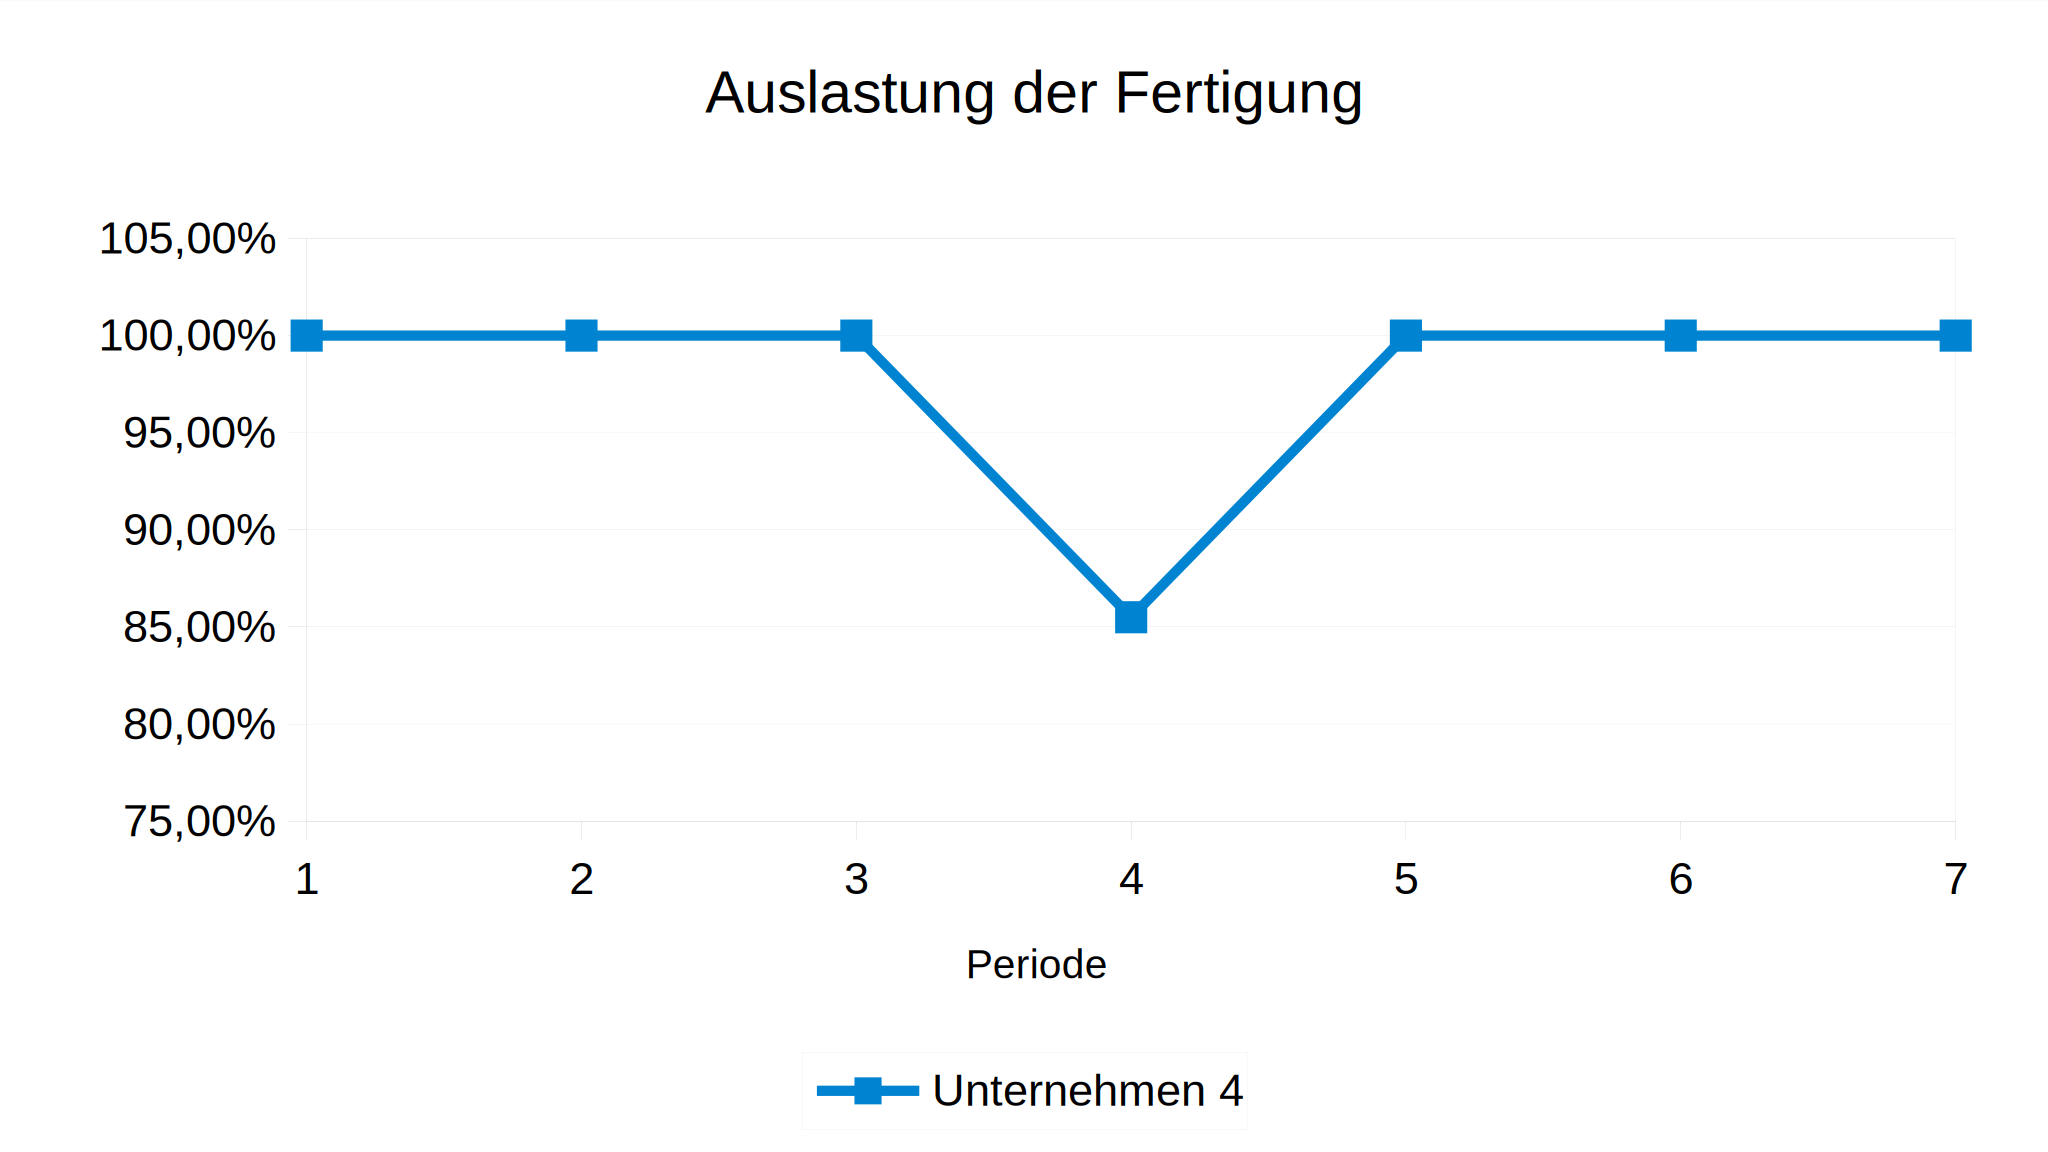
\includegraphics{./img/Auslastung_der_Fertigung.pdf}
 \caption[Auslastung der Fertigung]{Auslastung der Fertigung}
  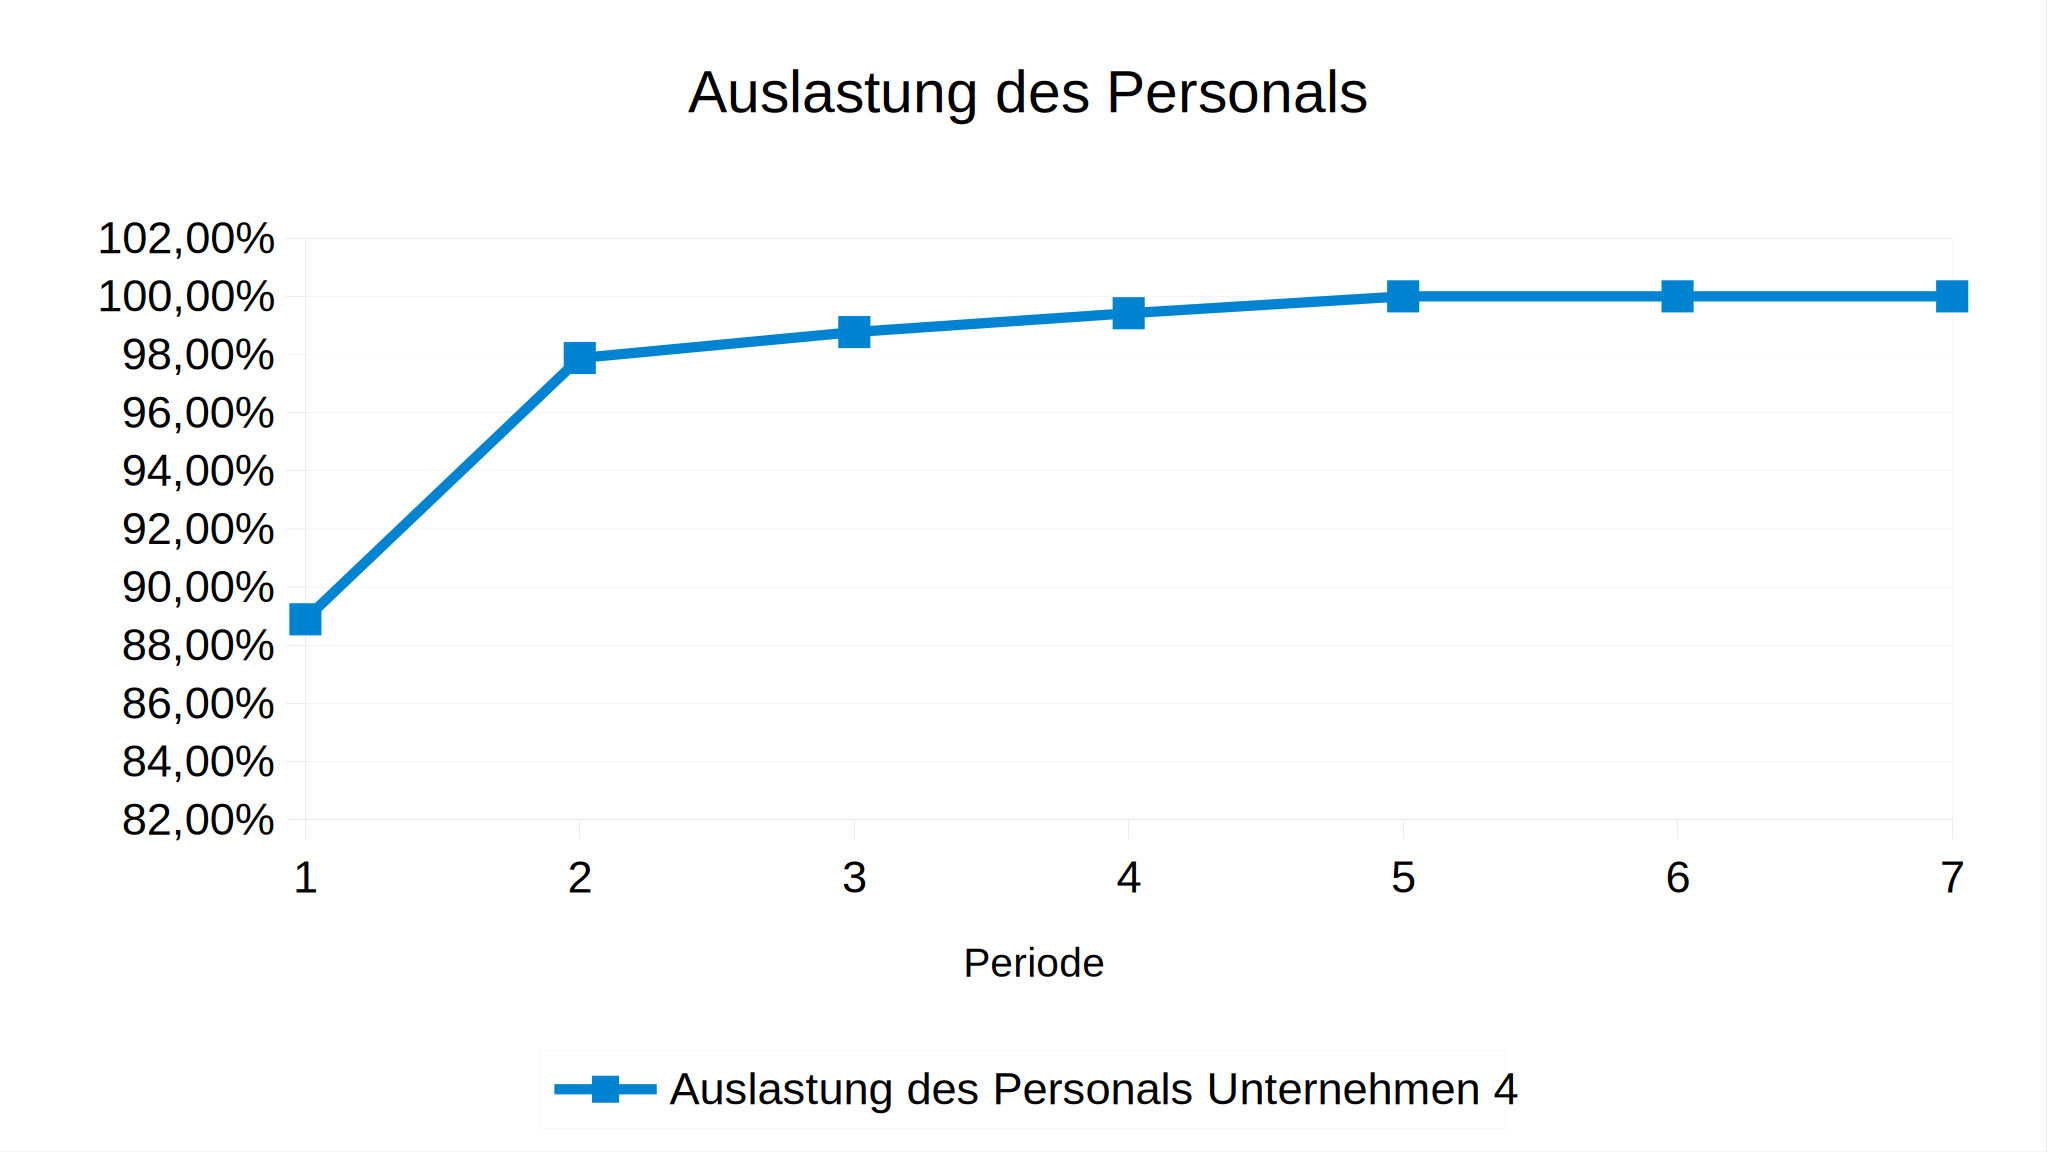
\includegraphics{./img/Auslastung_des_Personals.pdf}
  \caption[Auslastung des Personals]{Auslastung des Personals}  
\end{figure}

 
 \begin{figure}[th]
 \centering 
 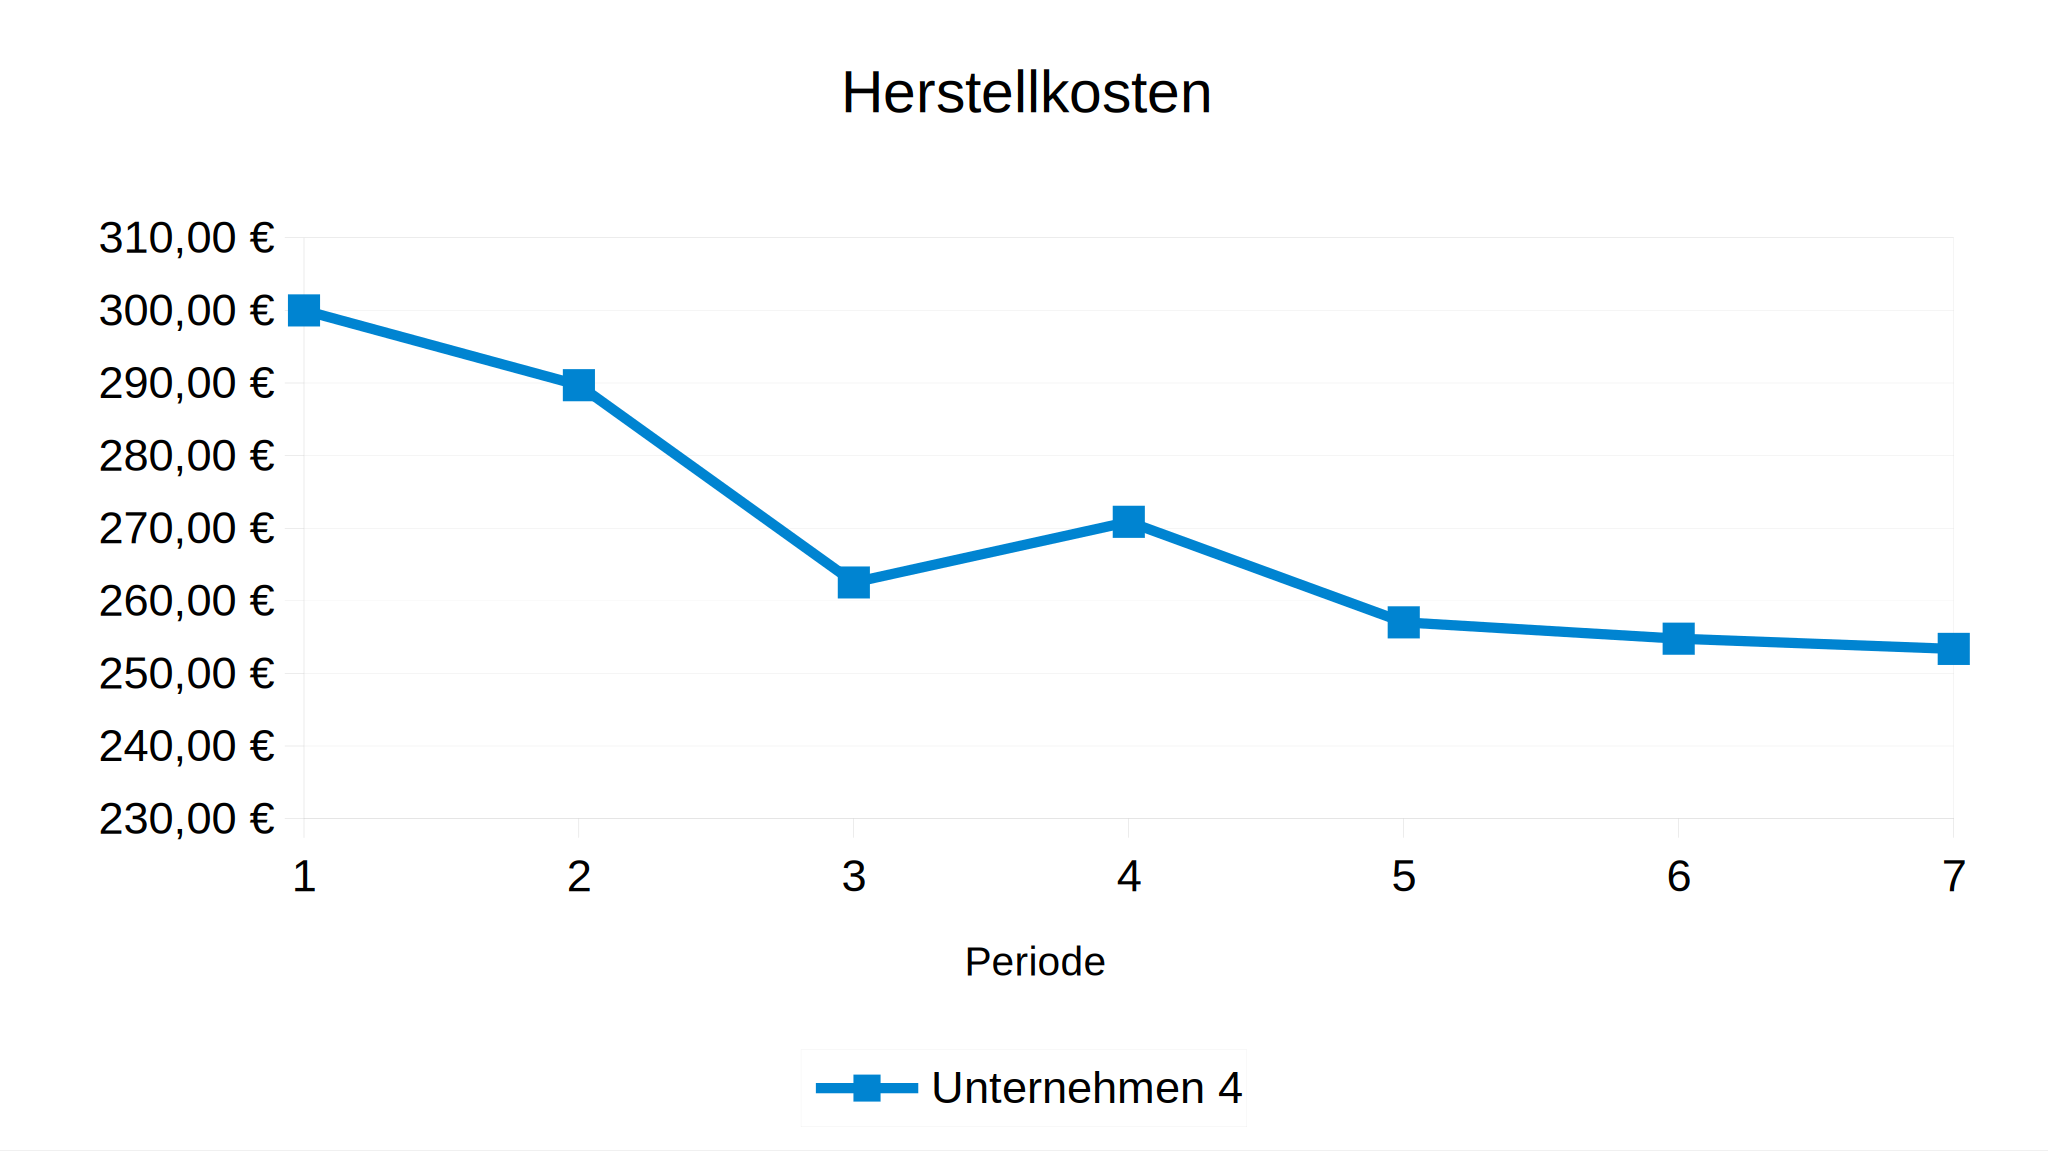
\includegraphics{./img/Herstellkosten.pdf}
  \caption[Herstellkosten]{Herstellkosten}
\begin{flushleft}
Wir waren in der Lage unsere Herstellkosten immer weiter zu senken. Dies war unter anderem möglich da wir die Auslastung des Personals auf 100\% erhöhen konnten. 
Der Anstieg der Herstellkosten in Periode 4 kommt daher, dass die Fertigungsanlagen nur bis zu 85\% ausgelastet waren.
In dieser Periode hatte ein Mitarbeiter gekündigt und die Neueinstellung von Mitarbeitern war in dieser Periode teurer als sonst.
Da wir einen hohen Lagerbestand an Zelten hatten, haben wir uns dazu entschlossen die Anlage für diese Periode mit geringer Auslastung zu betreiben und die Lager zu leeren.
\end{flushleft}
\end{figure}




 \begin{figure}[b]
 \centering 
 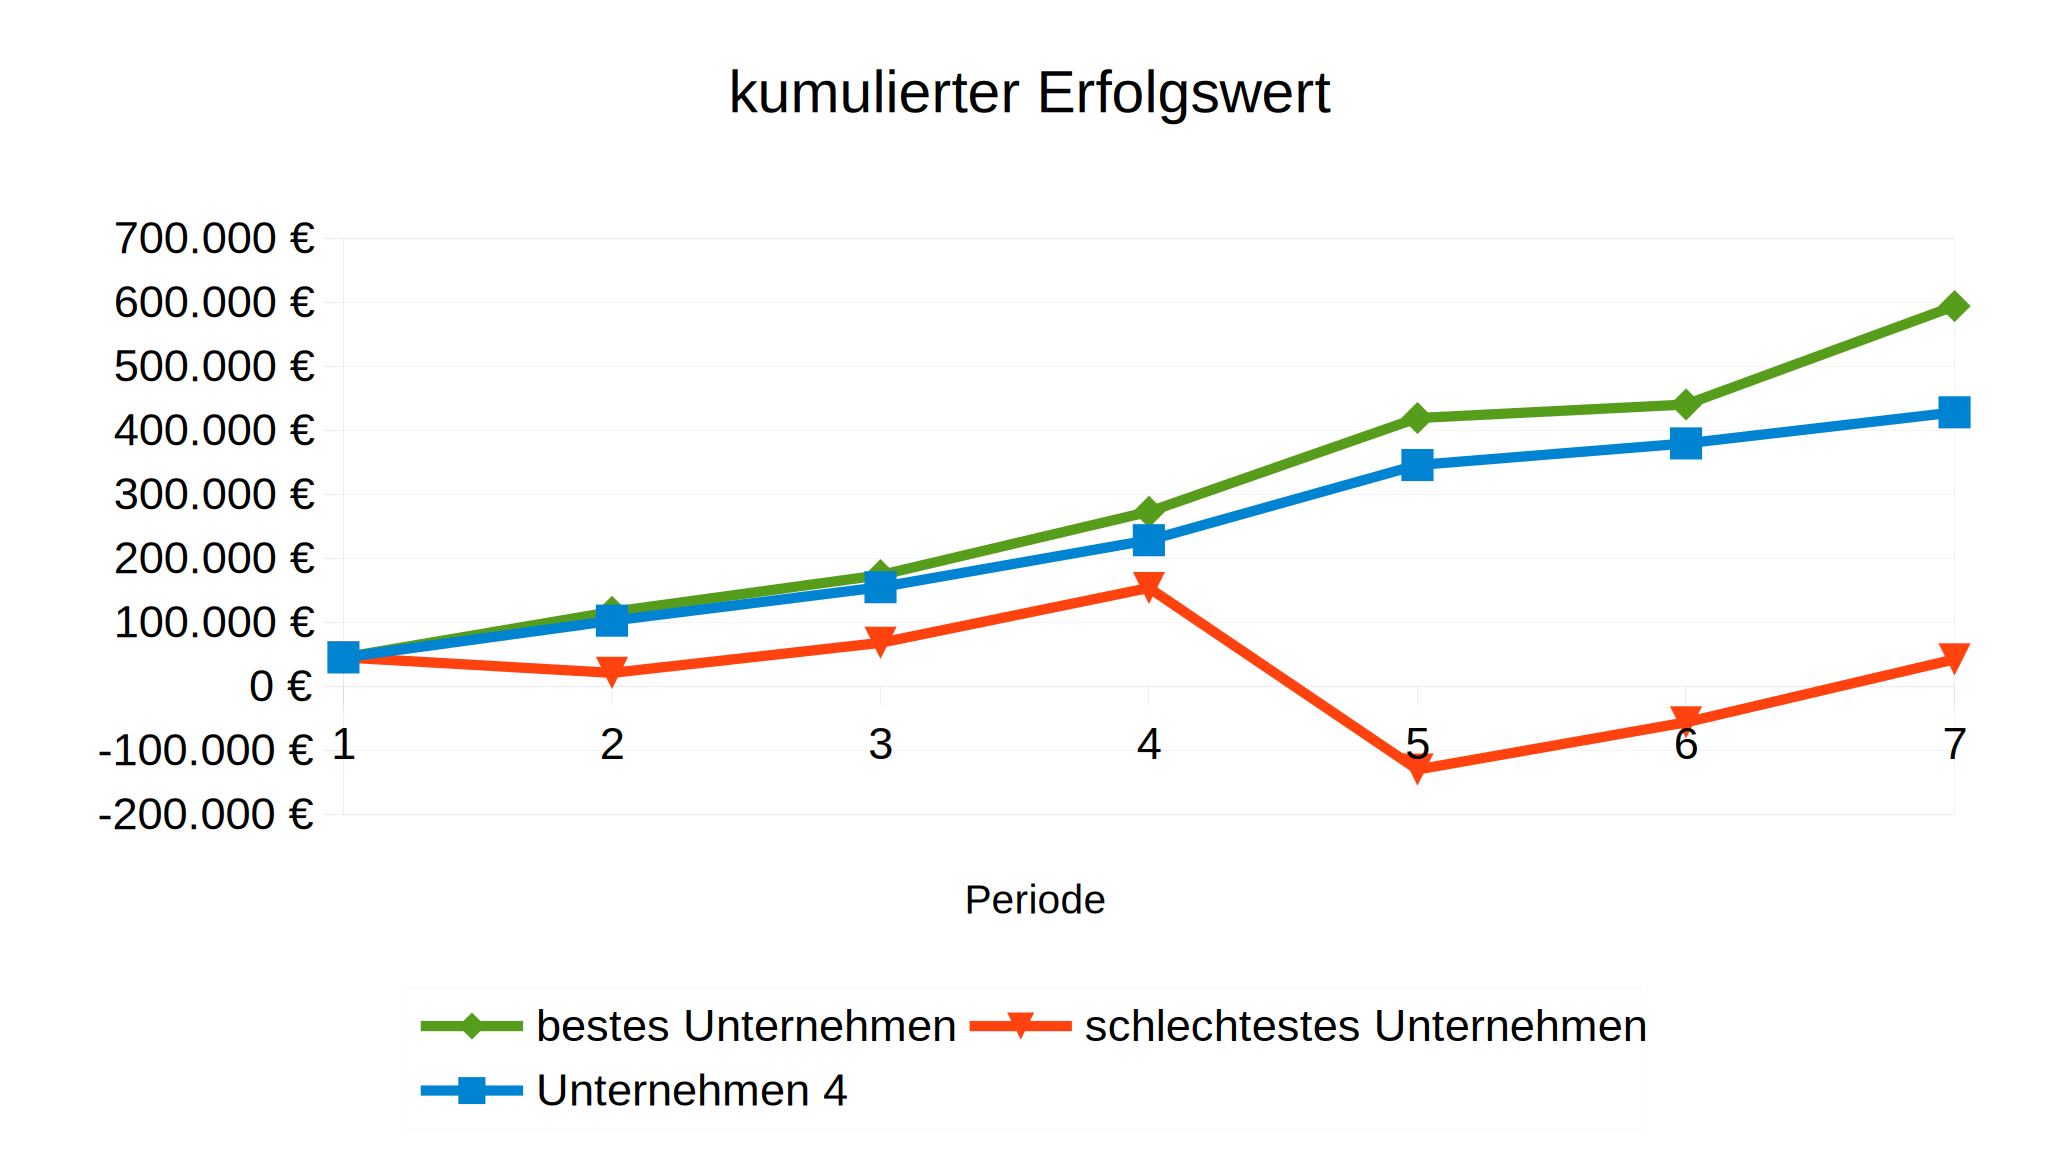
\includegraphics{./img/kumulierter_Erfolgswert.pdf}
  \caption[kumulierter Erfolgswert]{kumulierter Erfolgswert}
\end{figure}
 
 \begin{figure}
 \centering 
 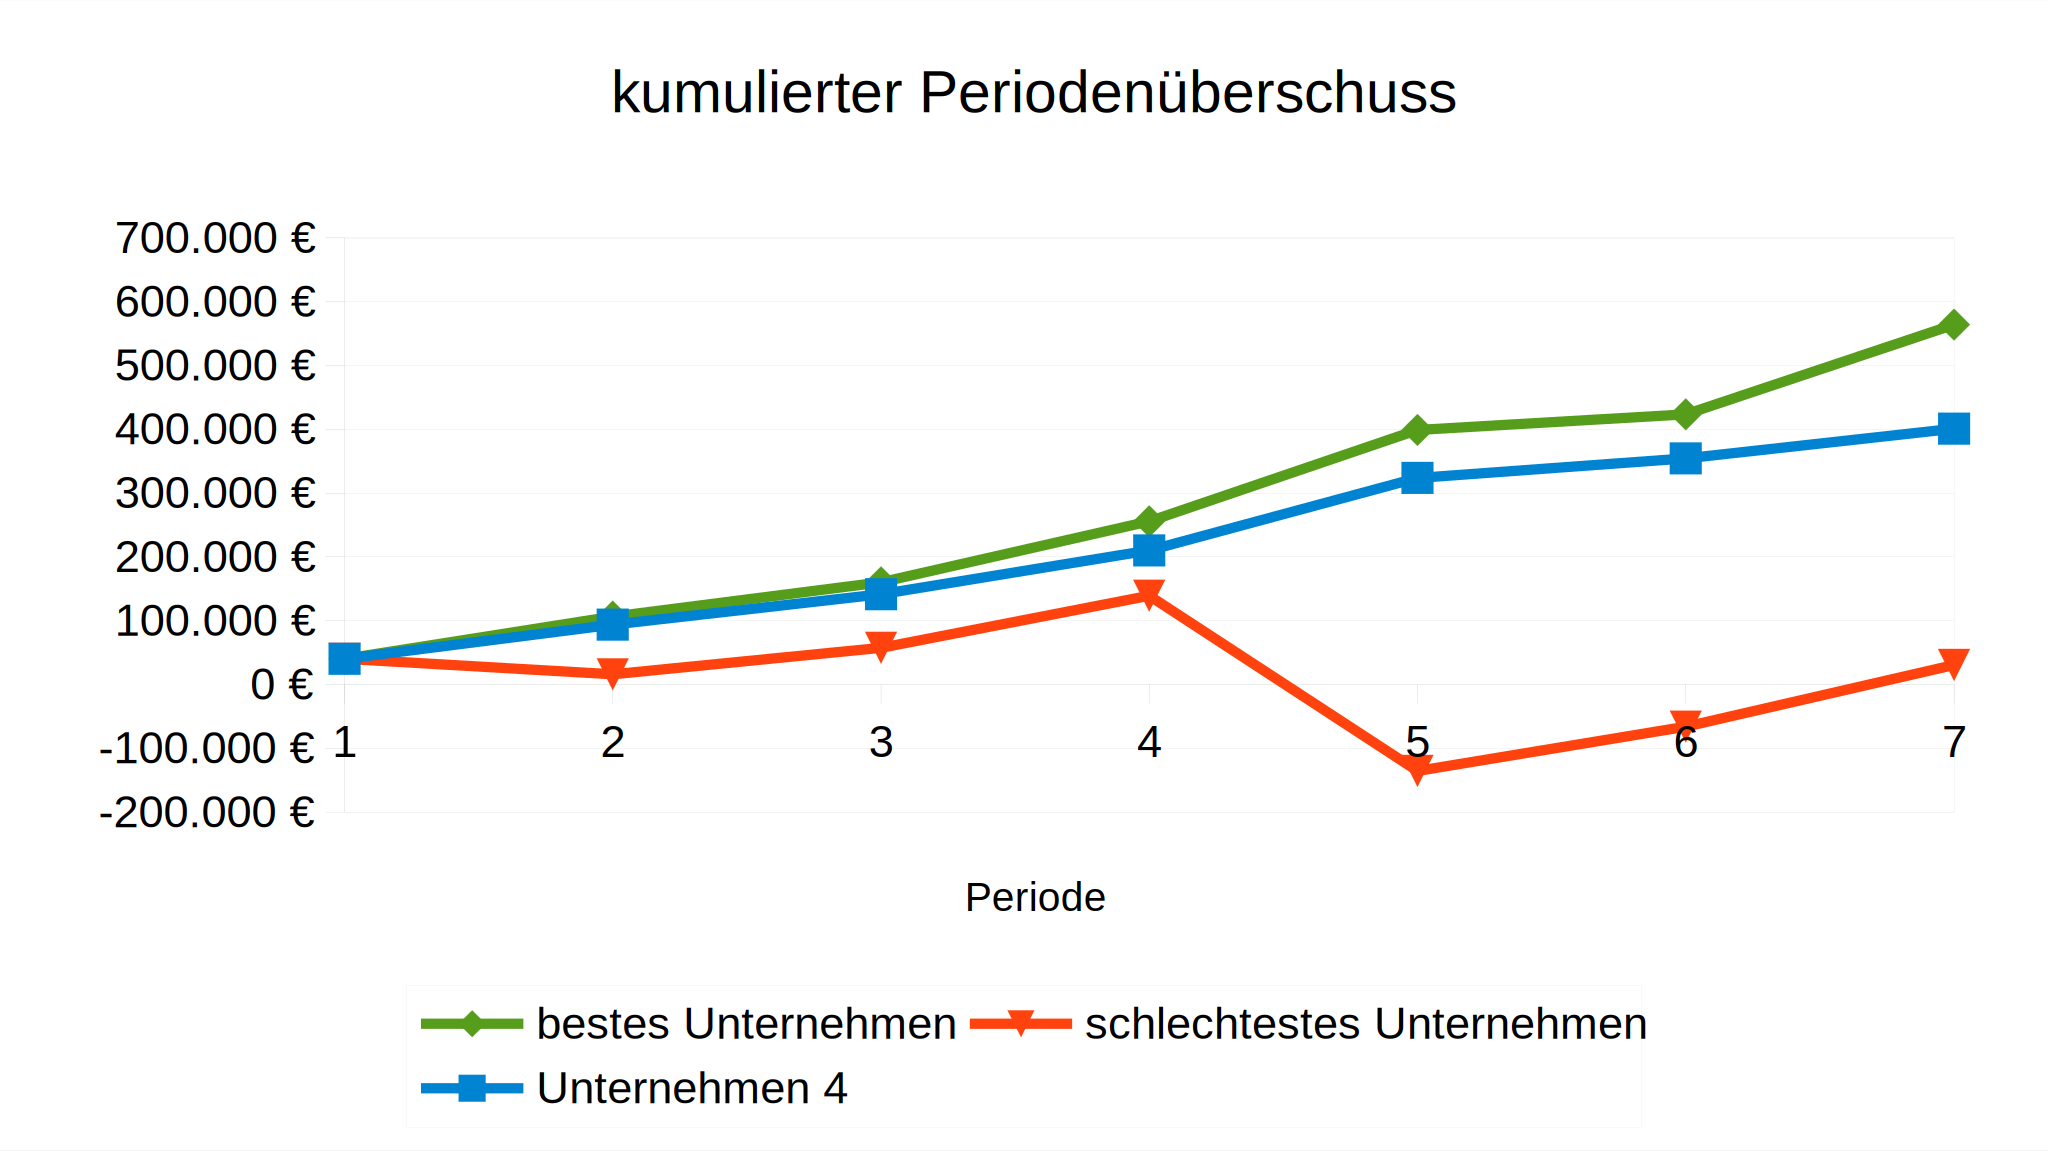
\includegraphics{./img/kumulierter_Periodenueberschuss.pdf}
  \caption[kumulierter Periodenüberschuss]
  {kumulierter Periodenüberschuss}
  \begin{flushleft}
In den ersten drei Perioden haben wir einen hohen Überschuss erzielt.
Dies gelang durch einen hohen Absatz und einen Preis von 450\texteuro pro Zelt. 
Dabei haben wir unter anderem von der Lieferunfähigkeit einiger Konkurrenten profitiert.
In den Folgeperioden haben wir versucht den Preis durch leichte Erhöhungen an den Markt anzupassen.
Unsere Entscheidung die Fertigungskapazitäten in Periode 4 nicht voll auszulasten erwies sich als Fehler.
Dadurch haben wir Überschuss eingebüßt. 
Für die letzte Periode hatten wir geplant den höchsten Absatz zu erzielen und erwarteten, dass die Konkurrenz das selbe Ziel hatte. Dies war jedoch nicht der Fall und wir setzten unseren Preis viel zu niedrig an, wodurch wir einen potentiellen Absatz von ca. 2500 Zelten hatte.
Zudem haben wir 600 Zelte an den Großhändler zu einem sehr günstigen Preis verkauft.
Unser niedriger Preis bewirkte eine große Nachfrage, die wir nicht befriedigen konnten.
So konnten die anderen Unternehmen ihre Zelte zu einem höheren Preis verkaufen.
  \end{flushleft}
\end{figure}

 \begin{figure}
 \centering 
 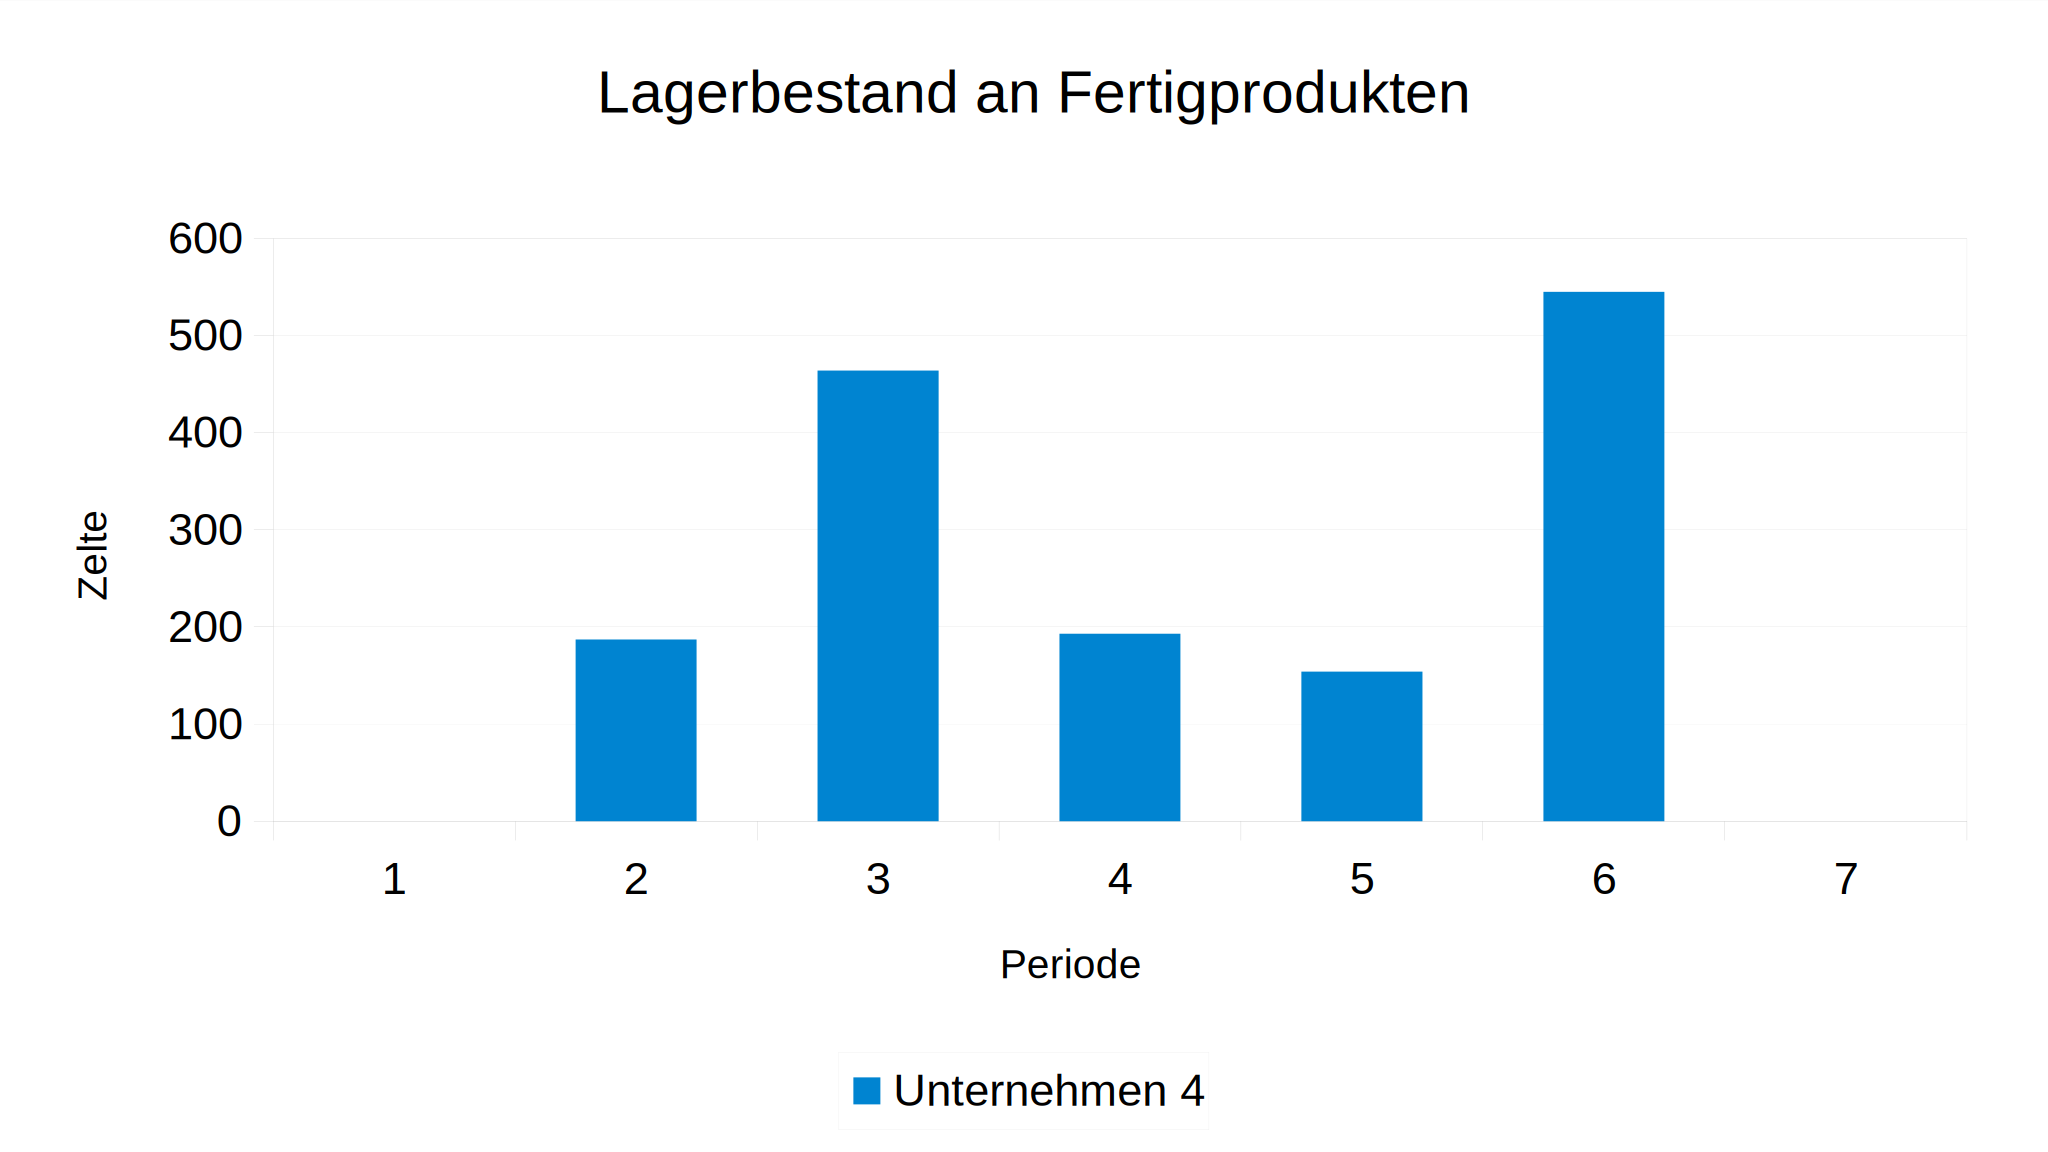
\includegraphics{./img/Lagerbestand_an_Fertigprodukten.pdf}
  \caption[Lagerbestand an Fertigprodukten]{Lagerbestand an Fertigprodukten}
\end{figure}

\begin{figure}
 \centering 
 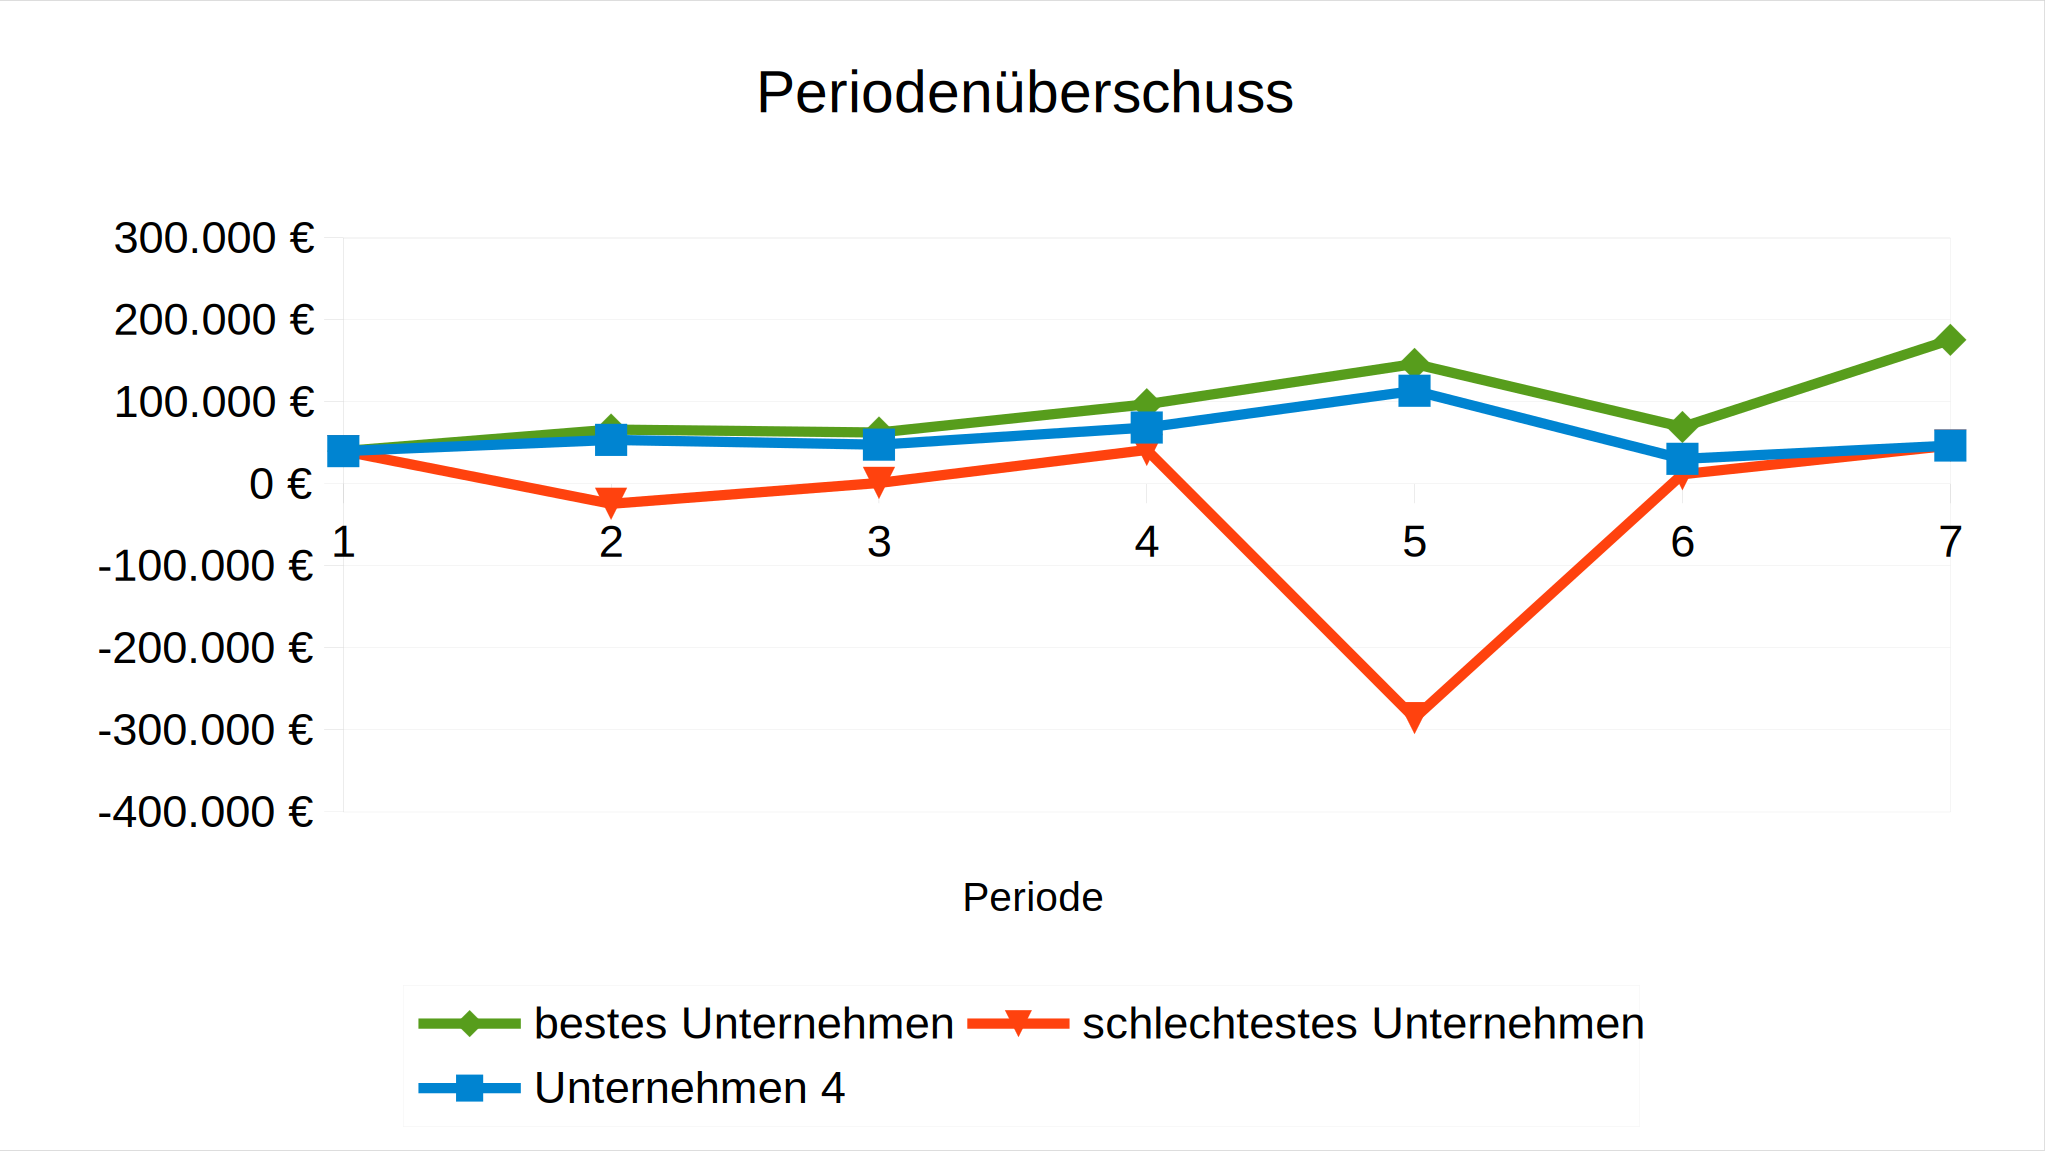
\includegraphics{./img/Periodenueberschuss.pdf}
  \caption[Periodenueberschuss]{Periodenueberschuss}
\end{figure}
 
 \begin{figure}[b]
 \centering 
 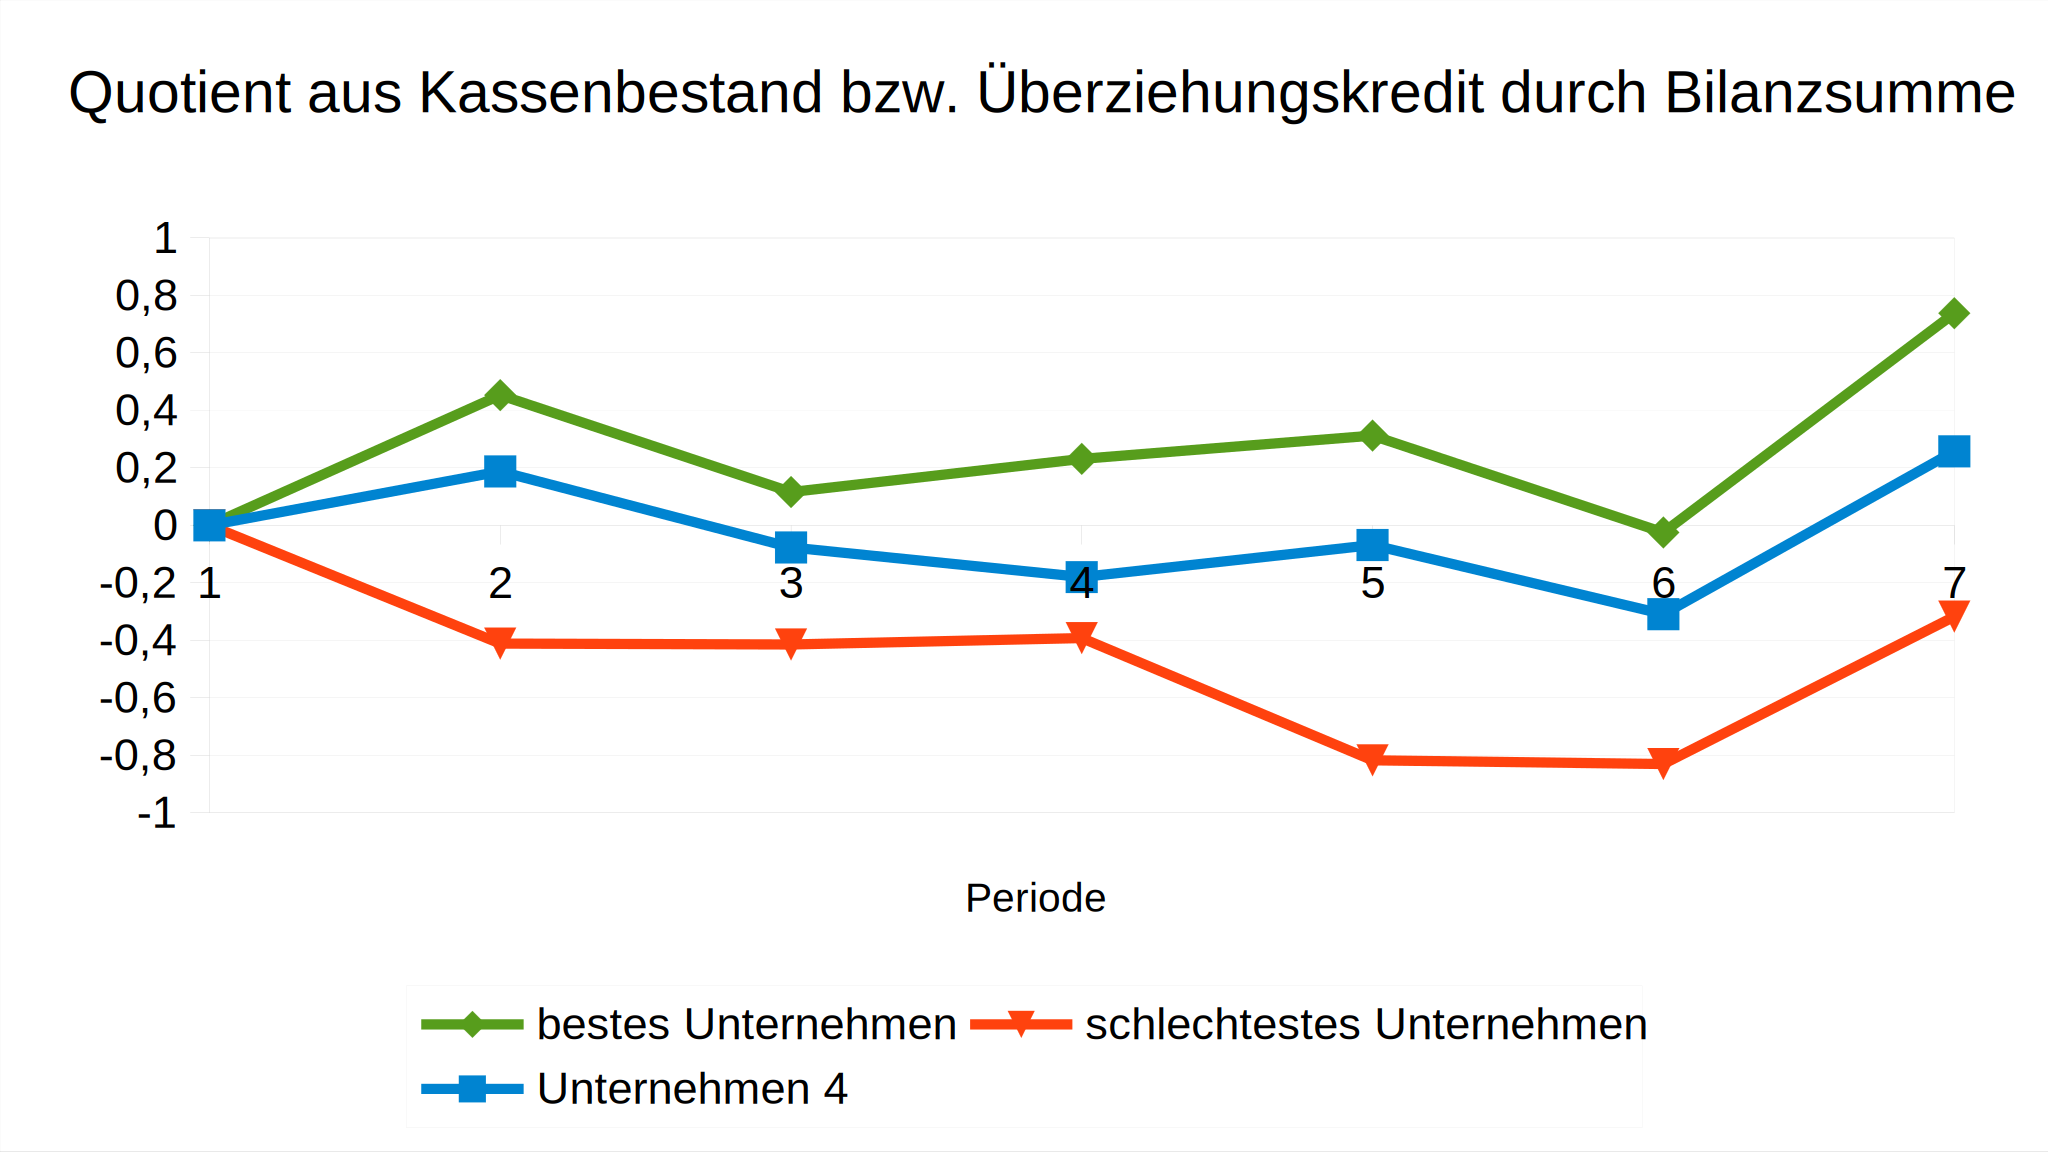
\includegraphics{./img/Quotient.pdf}
  \caption[Quotient]{Quotient}
\end{figure}



\chapter{Kritische Würdigung der Strategie}
Durch die frühe Anschaffung von Maschinen und Personal sowie des niedrigen Preises, war es uns schon früh möglich einen großen Absatz zu erzielen.
Unseren Preis haben wir immer an den aktuellen Markt sowie den Preisen der Konkurrenz angepasst um diese zu unterbieten ohne dabei die Qualität unseres Produktes zu vernachlässigen.
Leider haben wir einmal bei schwacher Konjunktur nicht genug Ware an den Markt bringen können wodurch wir unsere Überkapazität an den Großhändler zu einem viel niedrigerem Preis abtreten mussten.
Glücklicherweise konnten wir von der zu niedrigen Produktionskapazität verschiedener Unternehmen profitieren.
Zum Ende haben wir zwar mit einem sehr niedrigen Preis den größten Absatz erzielt aber unserer Produktion konnte nicht mit der Nachfrage mithalten.

\chapter{Die Situationsdarstellung des Unternehmens nach Periode 8}  
Im Nachhinein war unserer Preis zu niedrigen im Vergleich zur Menge der produzierbaren Zelte.
Unser potentieller Absatz an Zelten lag bei ca. 2500, wohingegen die unserer maximale Produktionskapazität lediglich bei 2000 lag.
Durch diese große Differenz konnten vor allem die anderen Unternehmen profitieren.
Für die nächste Periode würden wir unser Unternehmen um eine Anlage erweitern und zusätzliches Personal in der Produktion einstellen.
Damit wären wir in der Lage 2500 Zelte zu produzieren, was unserem aktuellem potentiellen Absatz entspricht.
Zudem hätten wir noch den Vorteile das wir den Mengenrabatt von Nylon und Gestänge besser ausnutzen könnten.

\chapter{Ausblick auf Periode 12}
Wir würden versuchen unseren Absatz von 2500 Zelten zu halten und evtl. auszubauen.
Einer unserer Fehler, den Großhändler mit in die Produktionsplanung mit einzubeziehen, würden wir nicht mehr wiederholen.
Ebenso würden wir bei bedarf unsere Produktionskapazität ausbauen, welches wir in den Vorperioden versäumt hatten.
Stattdessen würden wir ihn nur noch in schlechten Perioden nutzen um eine gesicherte Einnahmequelle zu erhalten und unseren Produktionsüberfluss zu kompensieren.


\chapter{Erfahrungen in und aus der Teamarbeit}
Da unsere Gruppe aus 3 Mitgliedern bestand war es einfach Entscheidungen zu treffen.
Da wir uns schnell auf ein Ziel einigen konnten, war die Entscheidungsfindung sehr einfach.
Ein Nachteil bei unserer Organisation war, dass nur eine Person aus der Gruppe Zugriff auf die Dropbox hatte.
Daher war diese Person dazu gezwungen immer da zu sein.
Das hätte zu einen Ausfall der Eingaben führen können, wäre die Person an einem Termin verhindert gewesen.
Im Nachhinein erwies es sich jedoch als positiv, denn es hat zu einer höheren Disziplin geführt, sodass alle Gruppenmitglieder sich intensiv mit der Planung beschäftigt haben und die Entscheidungen schon im Voraus getroffen und abgeschickt wurden.
Eine strikte Aufgabenteilung gab es während des Planspiels nicht.
Zusammenfassend kann man sagen dass die Gruppenarbeit sehr gut lief.
Einziger Vierbesserungspunkt wäre ein gemeinsamer Zugriff zur Dropbox. 

\chapter{Anhang}



Die Pflichtinhalte ergeben sich aus den nachfolgenden Gliederungspunkten.
Prognoserechnung
Absatz- und Produktionsplanung
Kostenrechnung
Finanzplanung
Ergebnisplanung (GuV)

%
%%\begin{figure}[htbp]
%\centering
%\includesvg[width=1\textwidth]{./Auslastung_der_Fertigung2}
%	\caption{Auslastung der Fertigung}
%%  \caption{svg NewTux}
%\end{figure}


%
% \begin{figure}
% \centering 
% \includegraphics[pages={1}]{./img/TopSim_Anhang.pdf}
%\end{figure}
 
%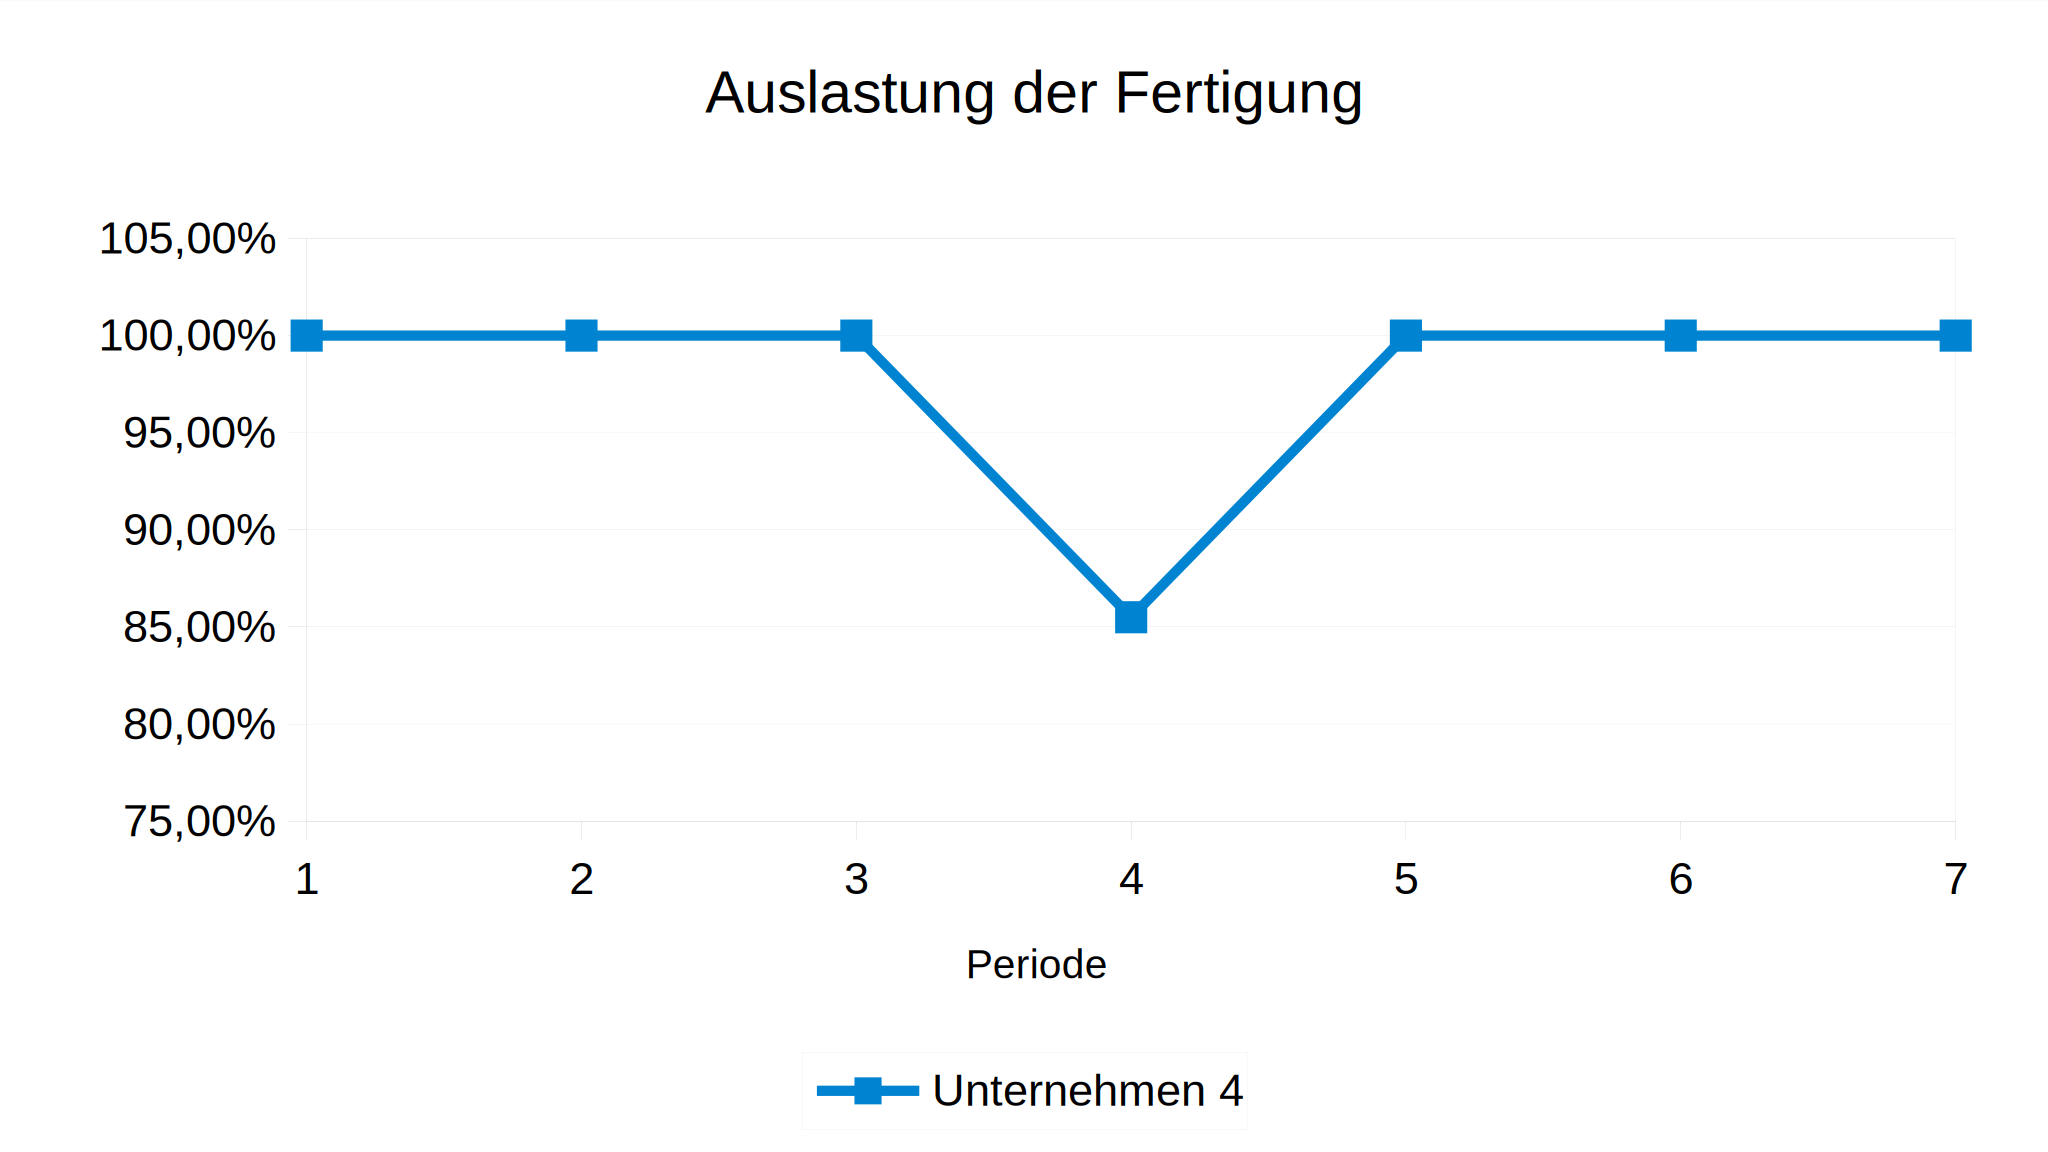
\includepdf[noautoscale]{./img/Auslastung_der_Fertigung.pdf}
%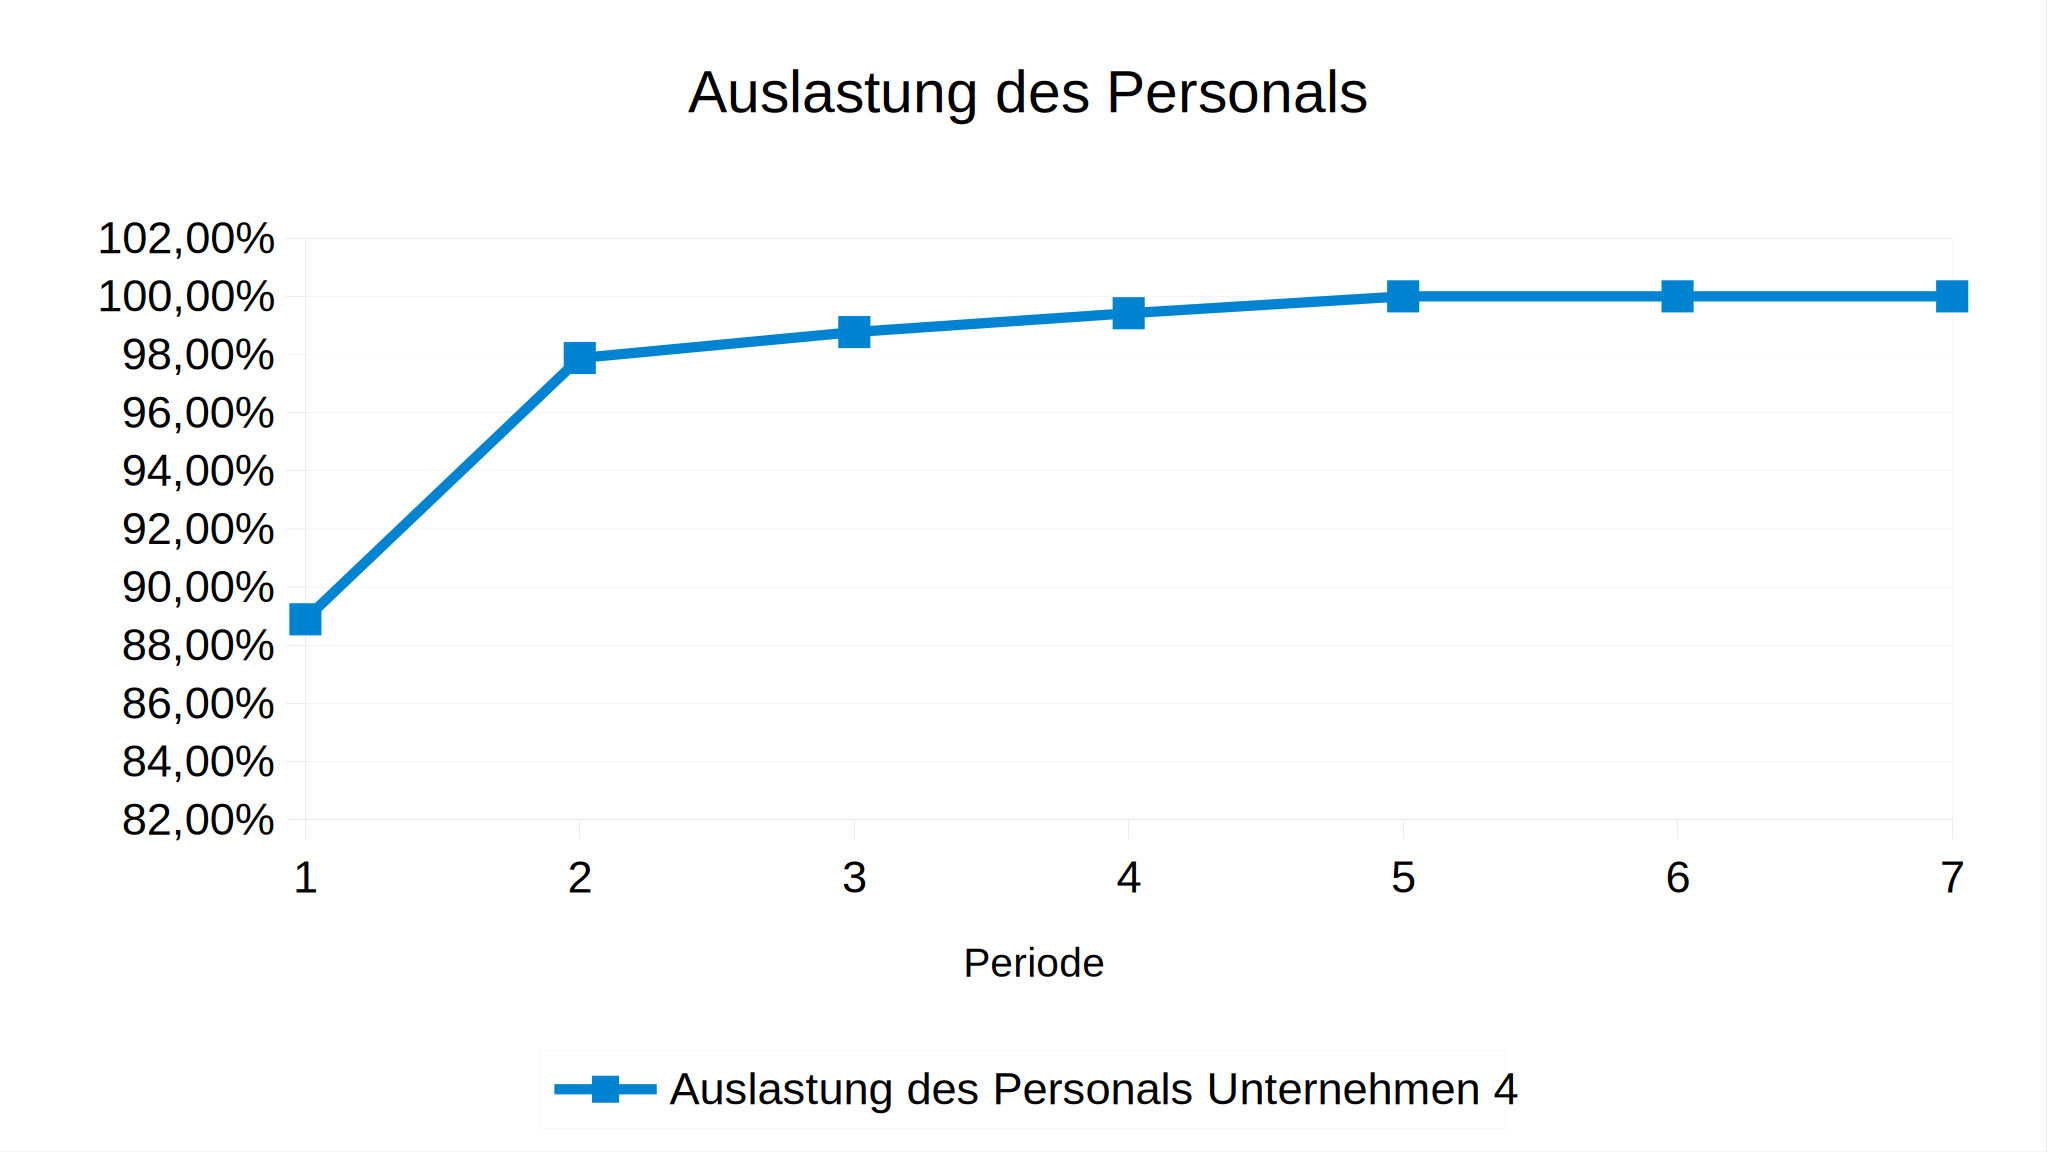
\includepdf[noautoscale]{./img/Auslastung_des_Personals.pdf}
%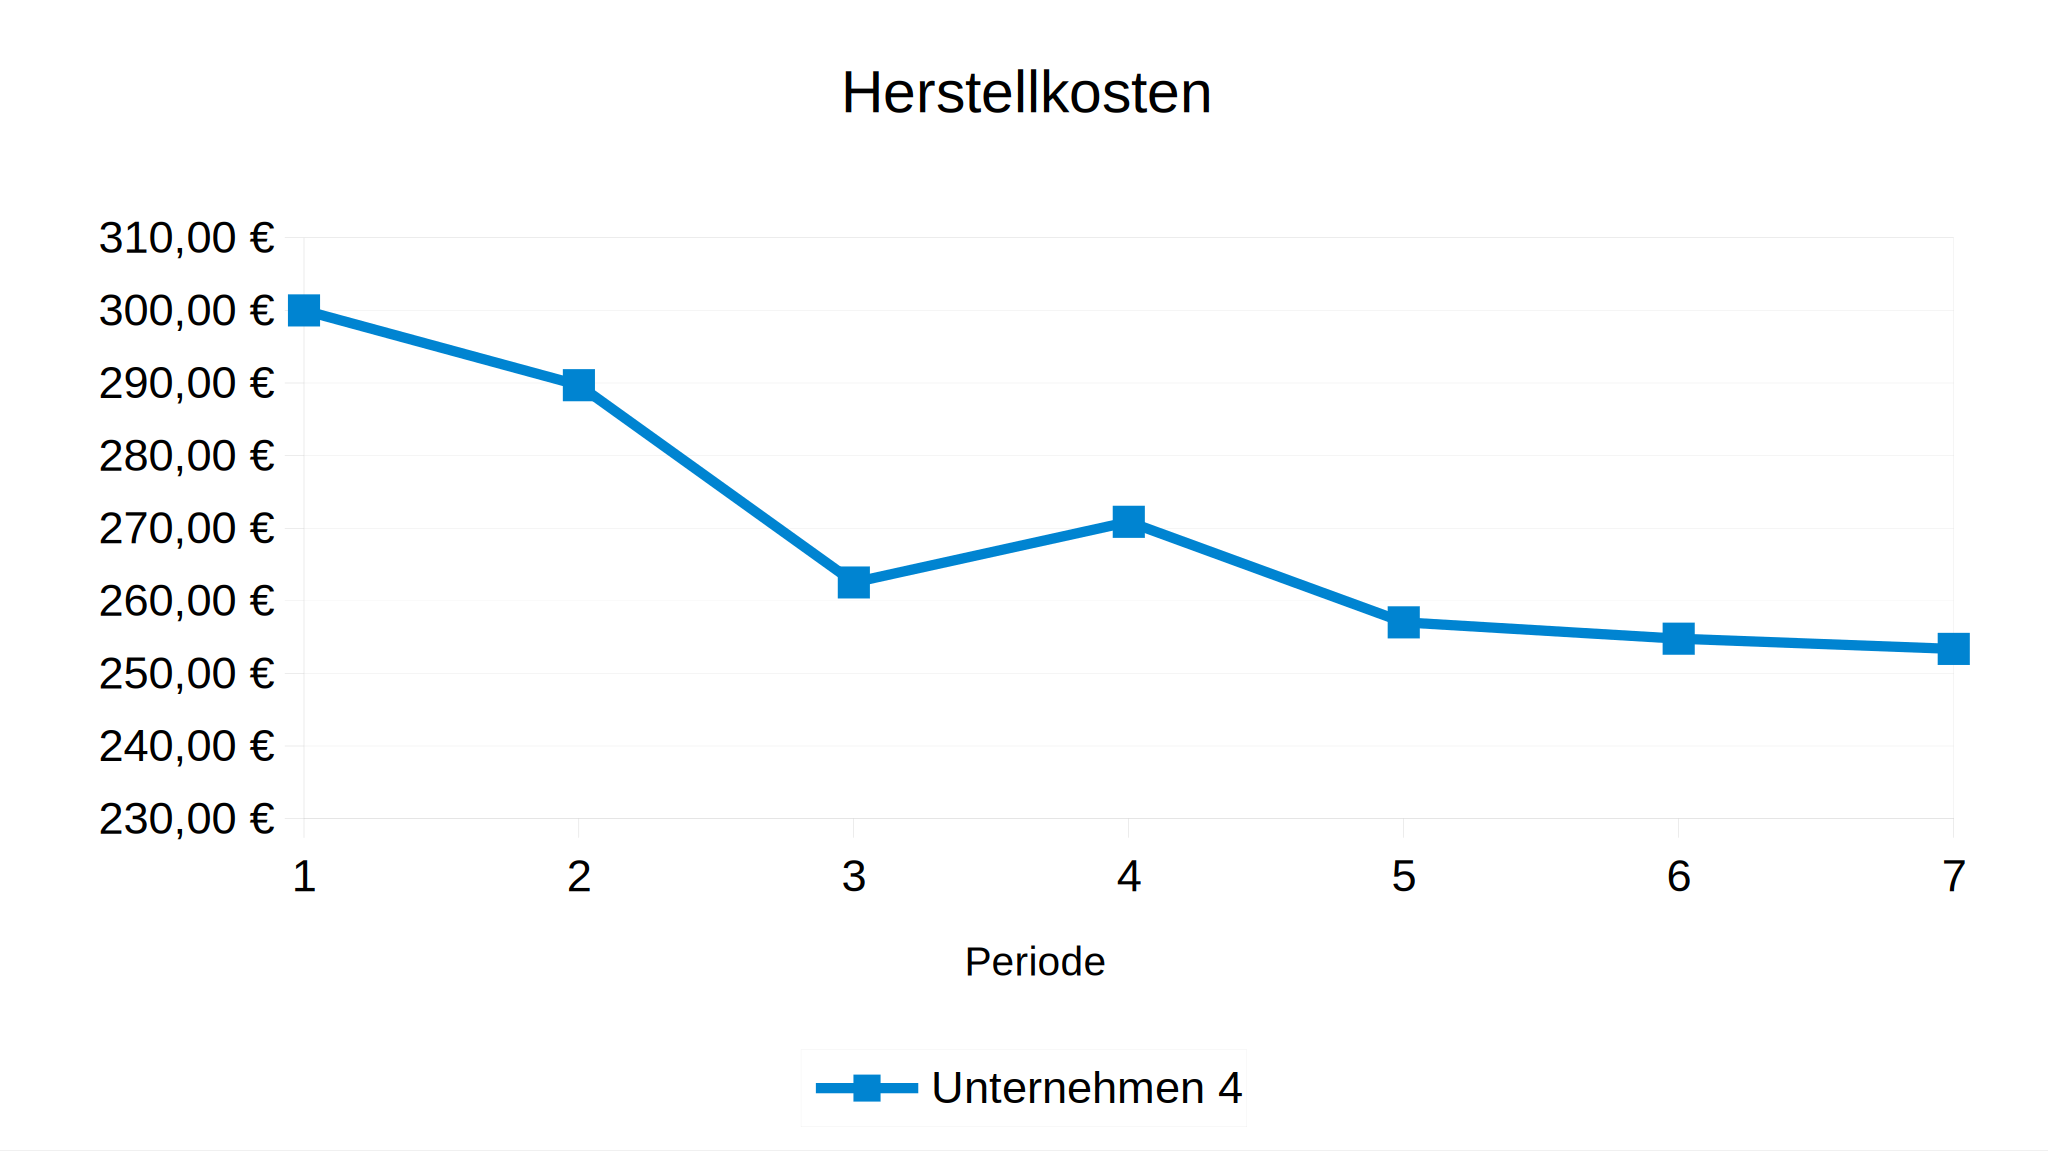
\includepdf[noautoscale]{./img/Herstellkosten.pdf}
%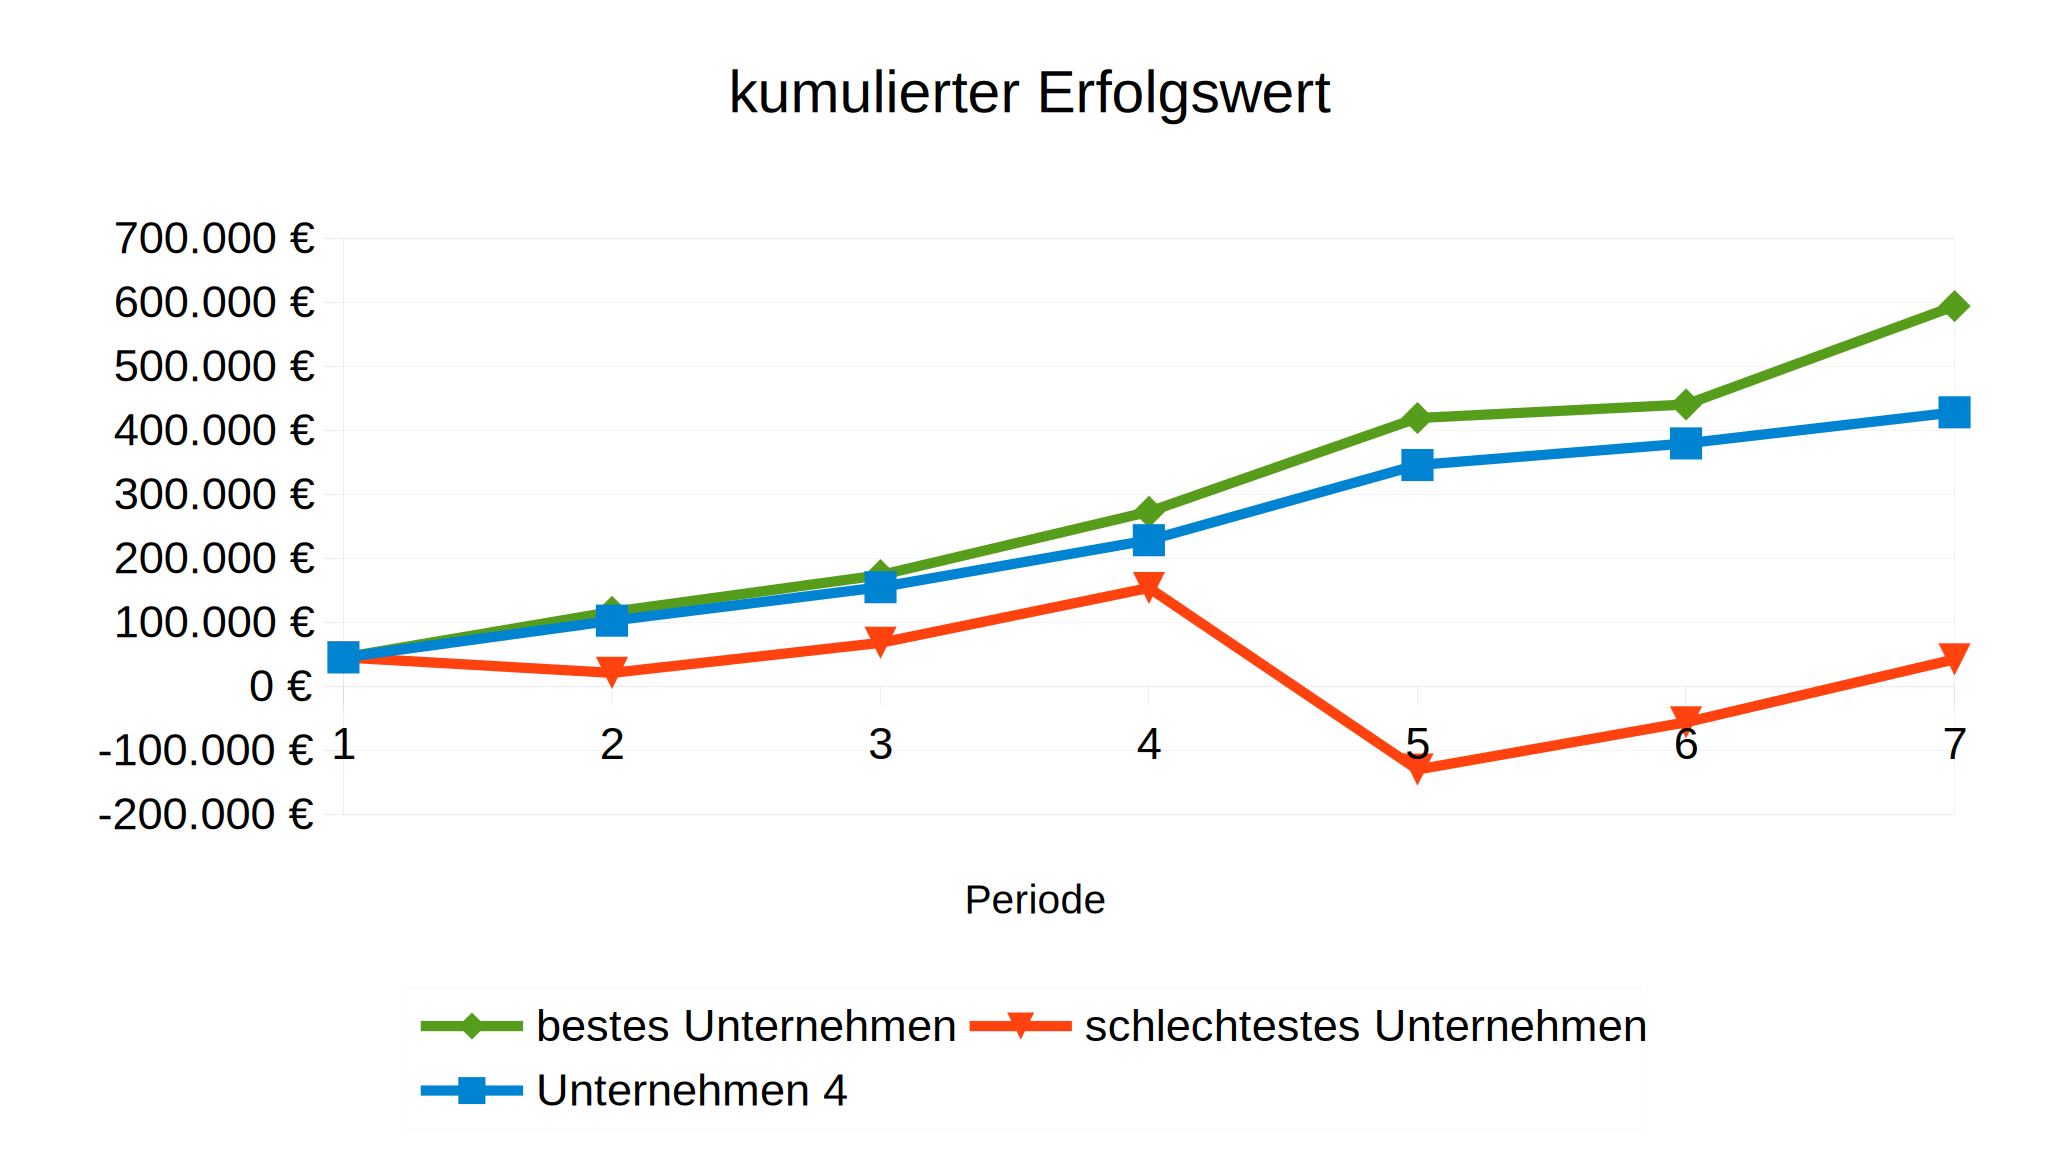
\includepdf[noautoscale]{./img/kumulierter_Erfolgswert.pdf}
%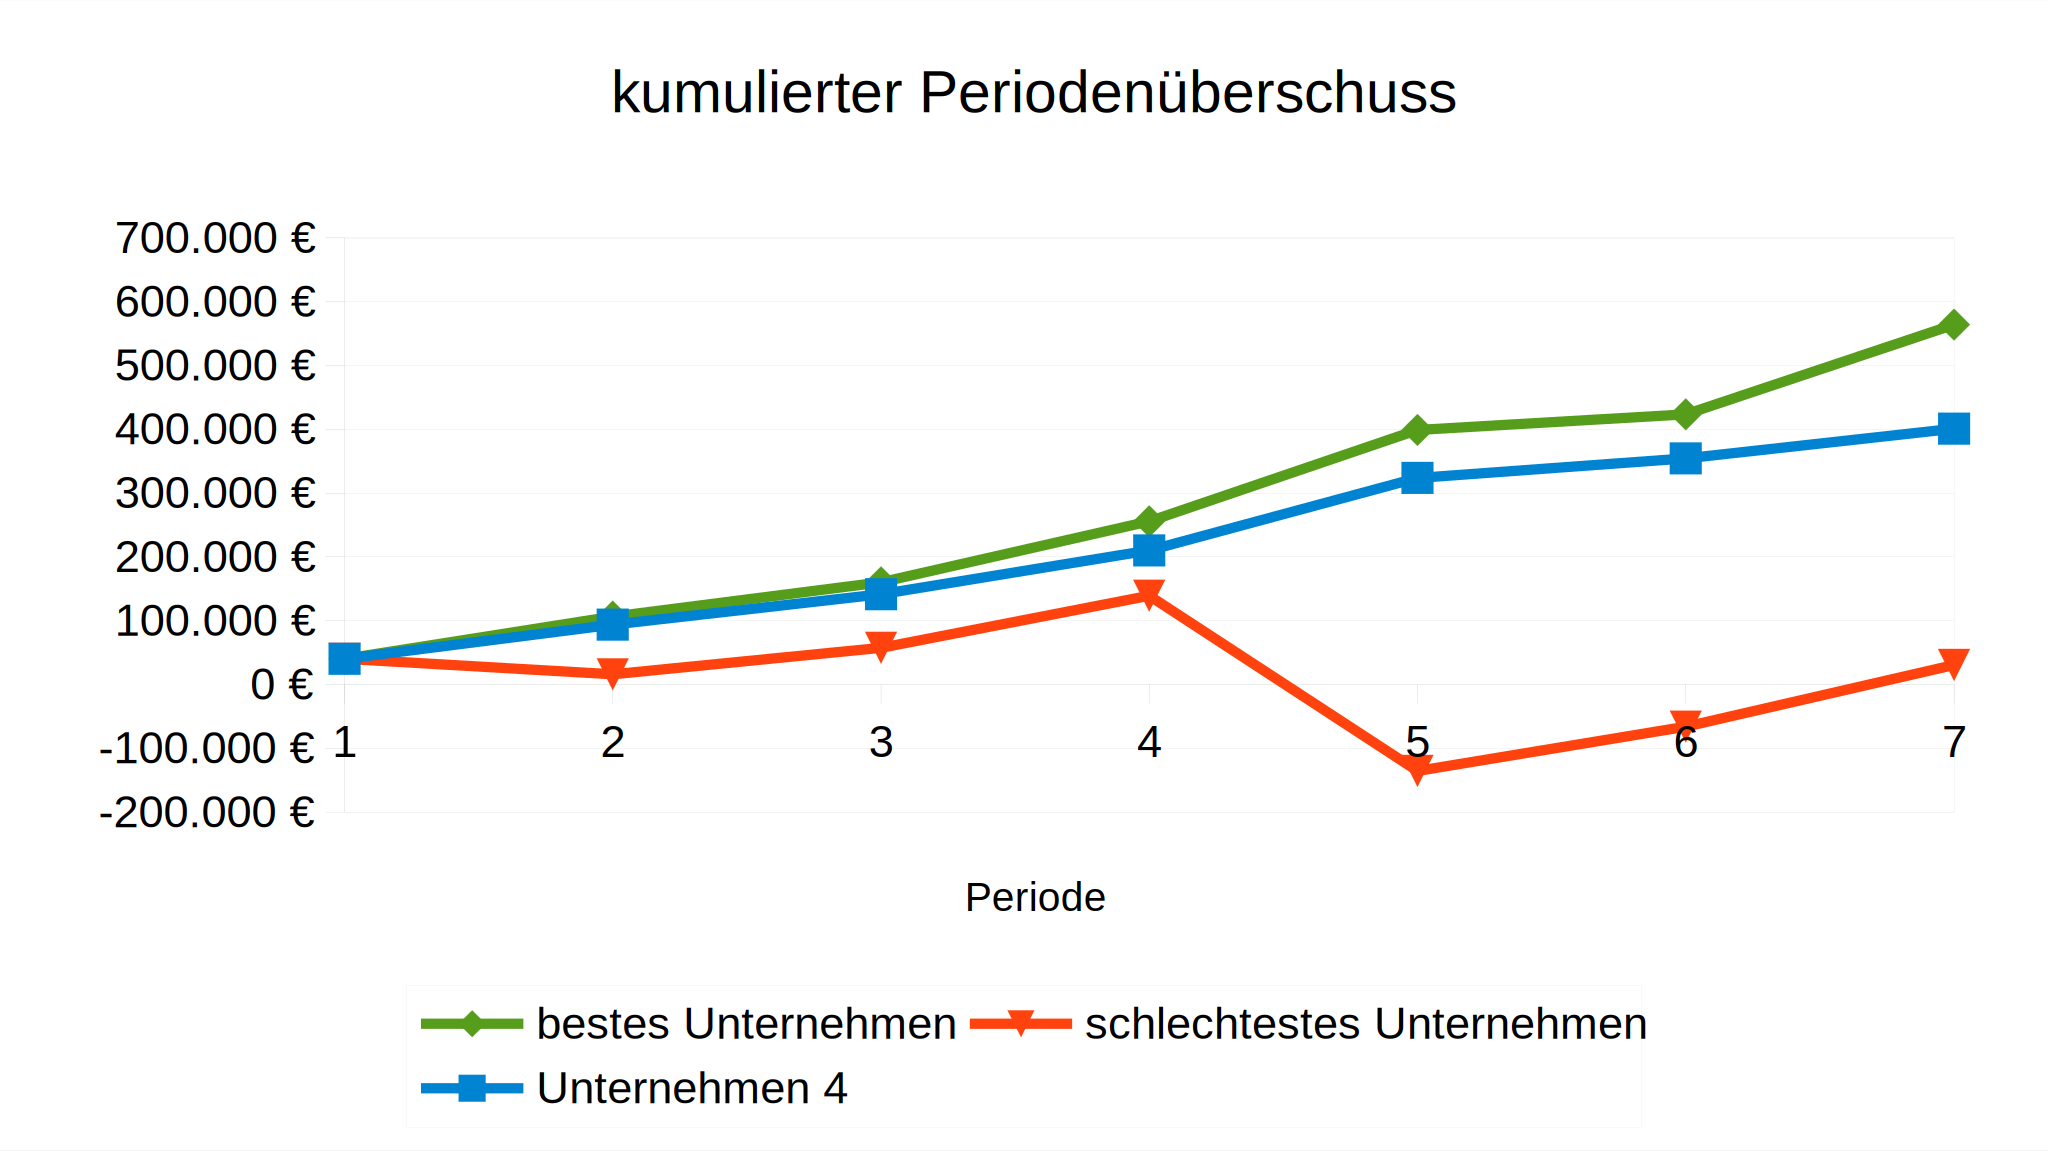
\includepdf[noautoscale]{./img/kumulierter_Periodenueberschuss.pdf}
%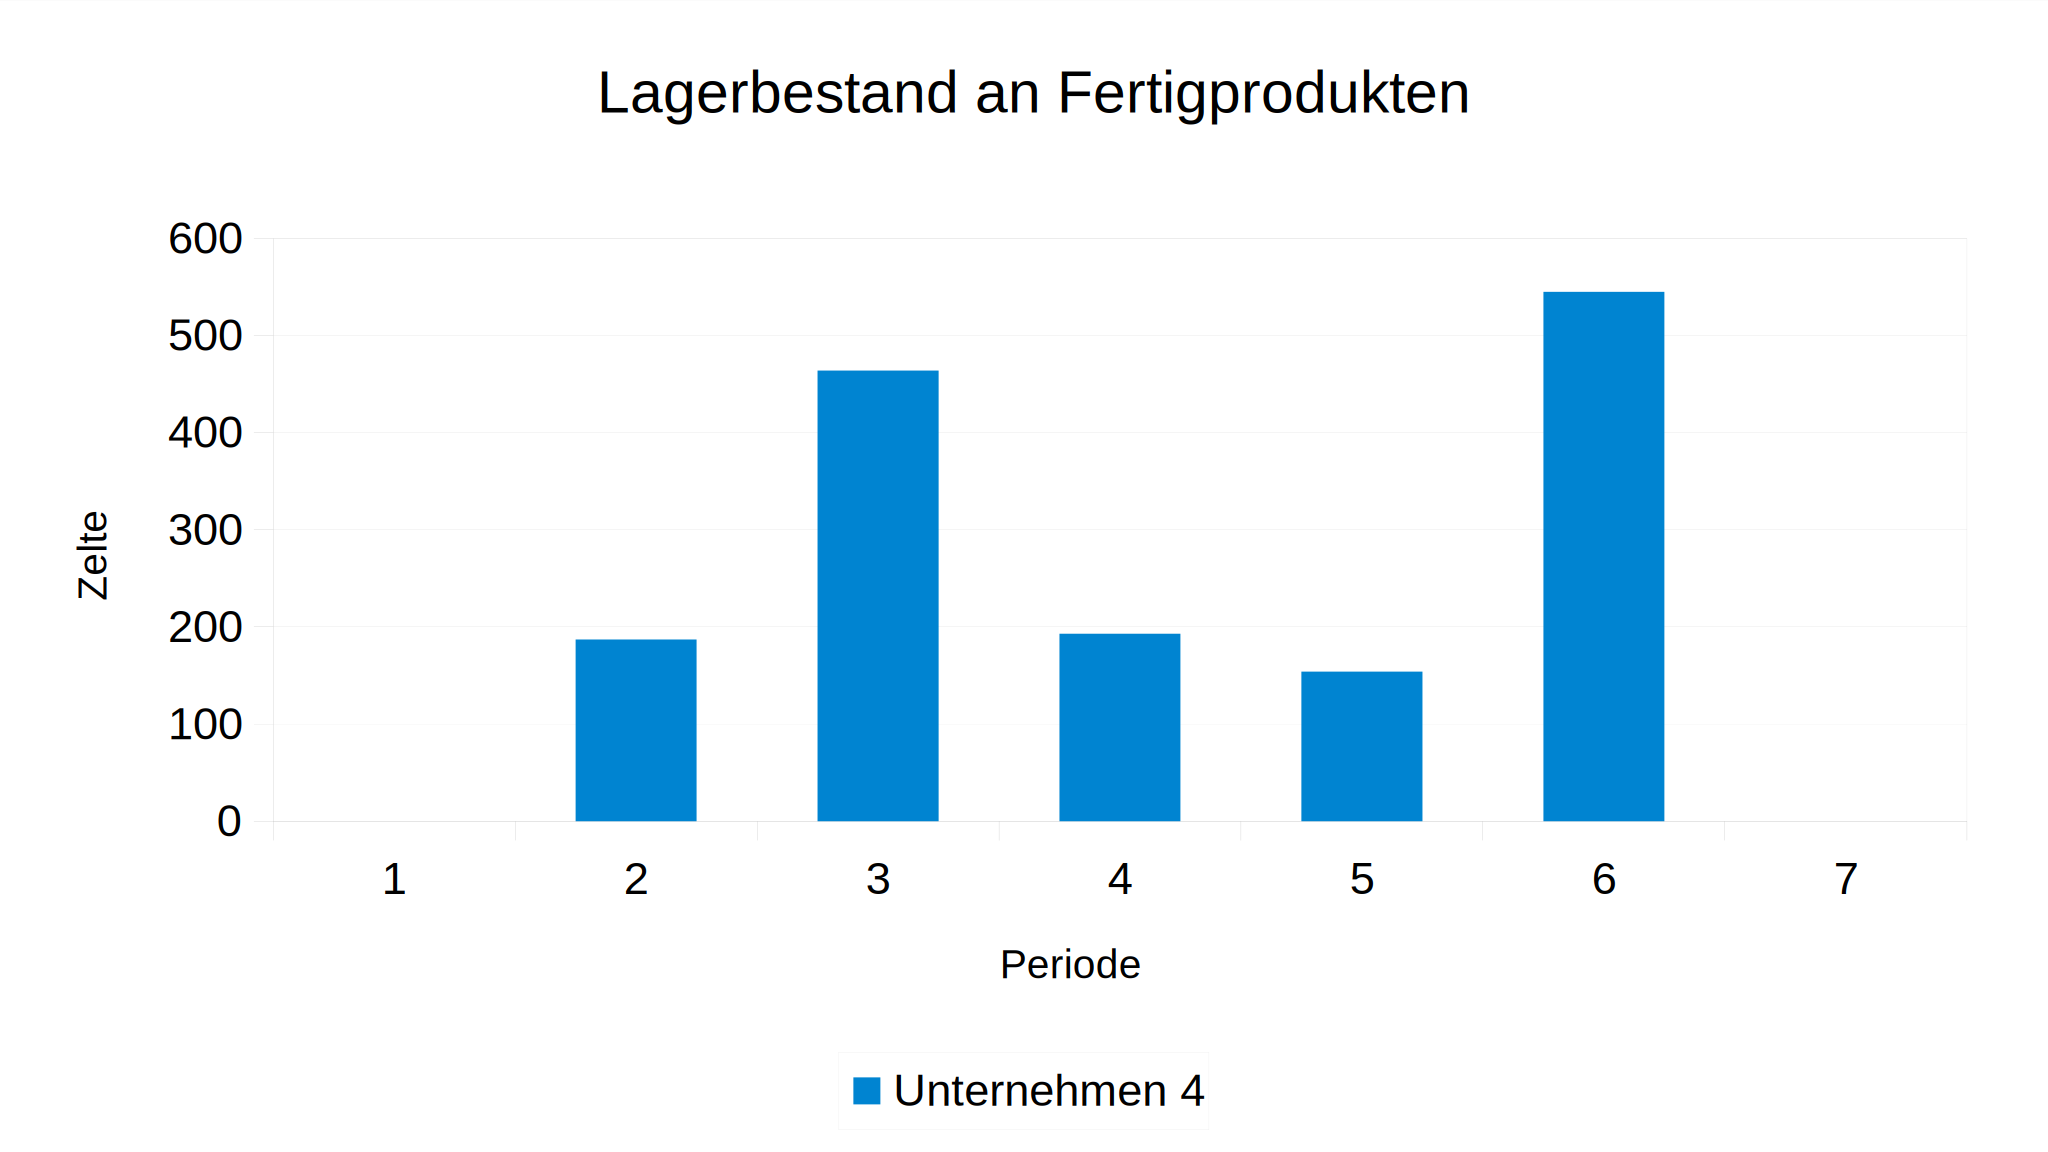
\includepdf[noautoscale]{./img/Lagerbestand_an_Fertigprodukten.pdf}
%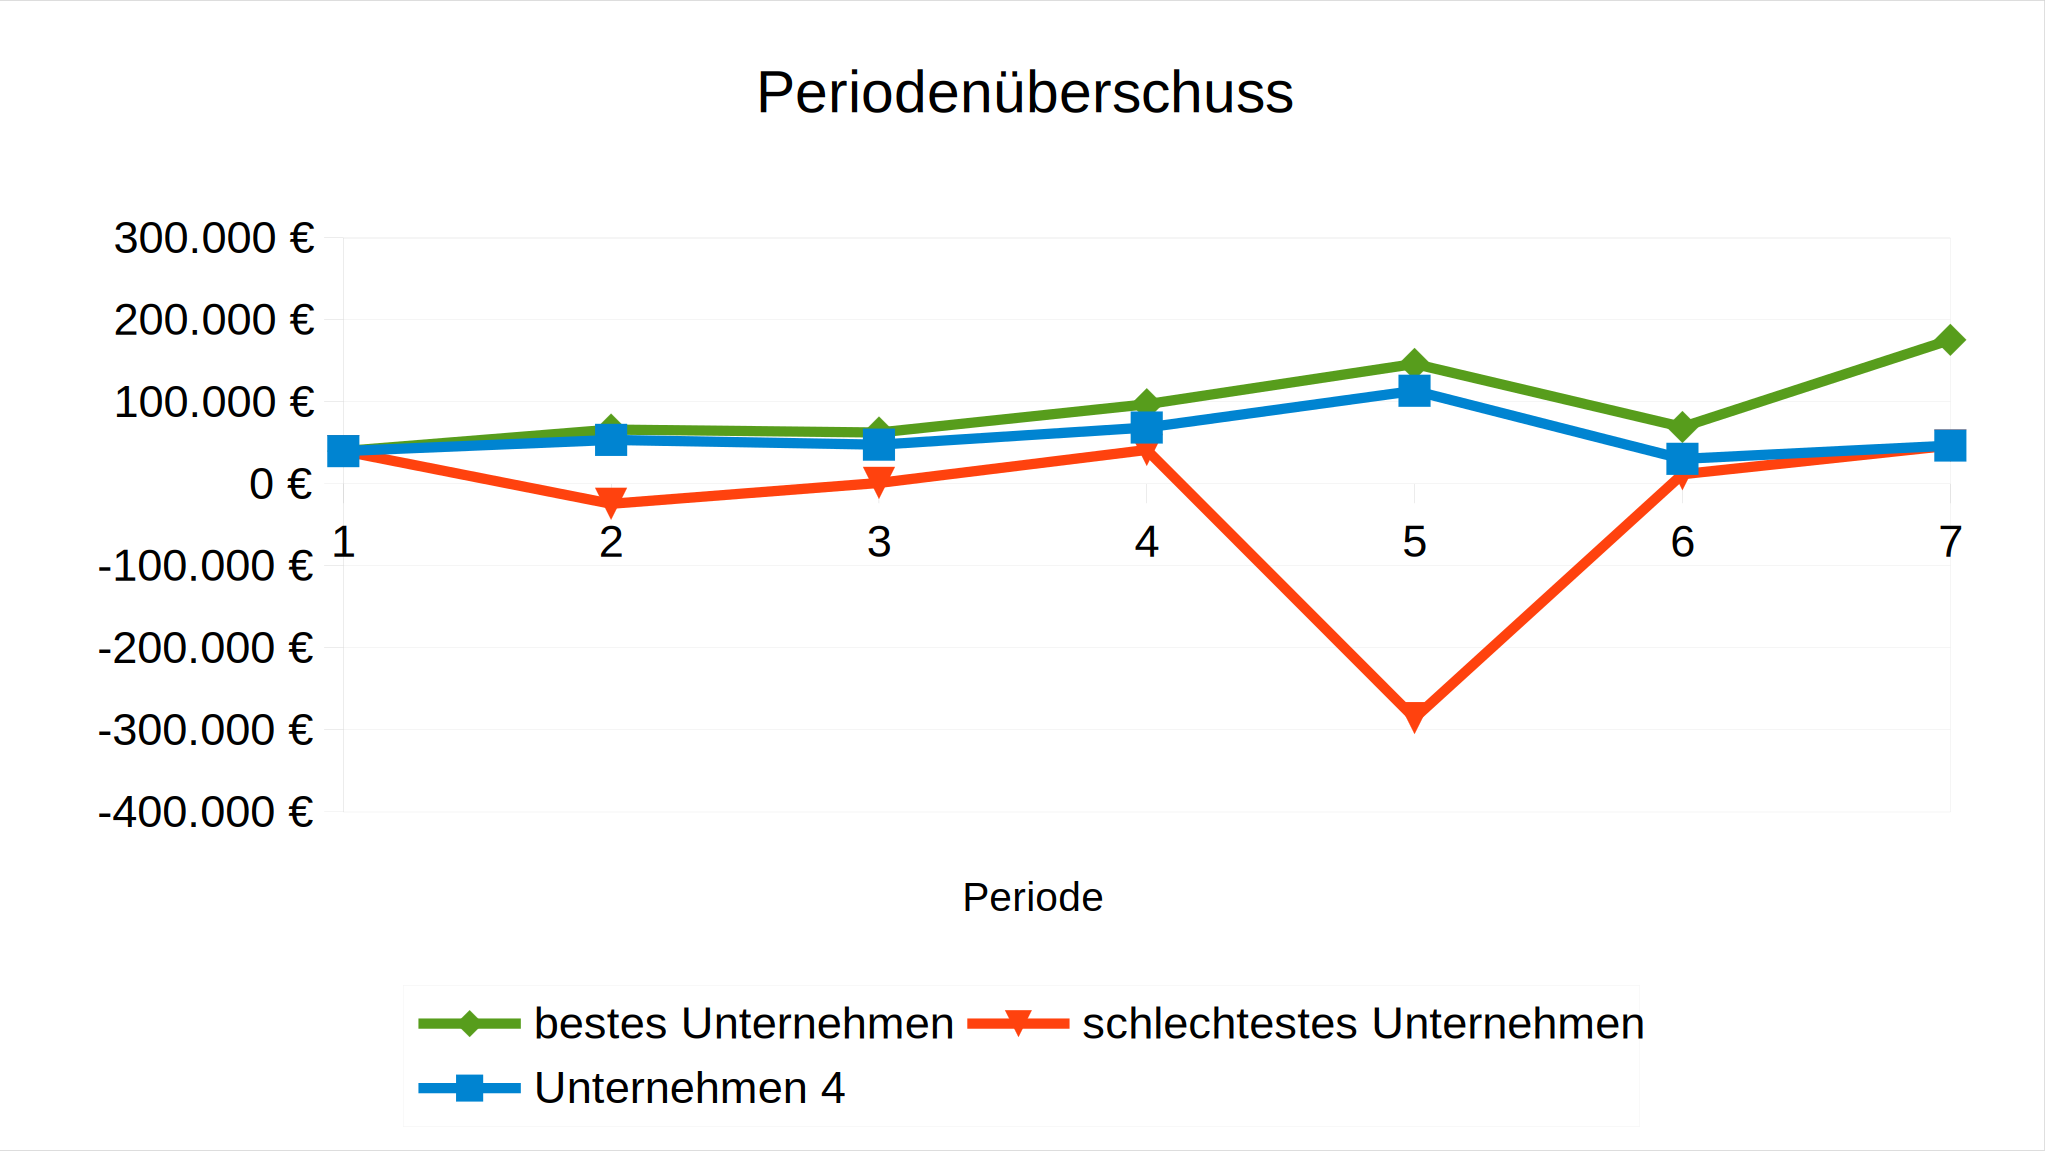
\includepdf[noautoscale]{./img/Periodenueberschuss.pdf}
%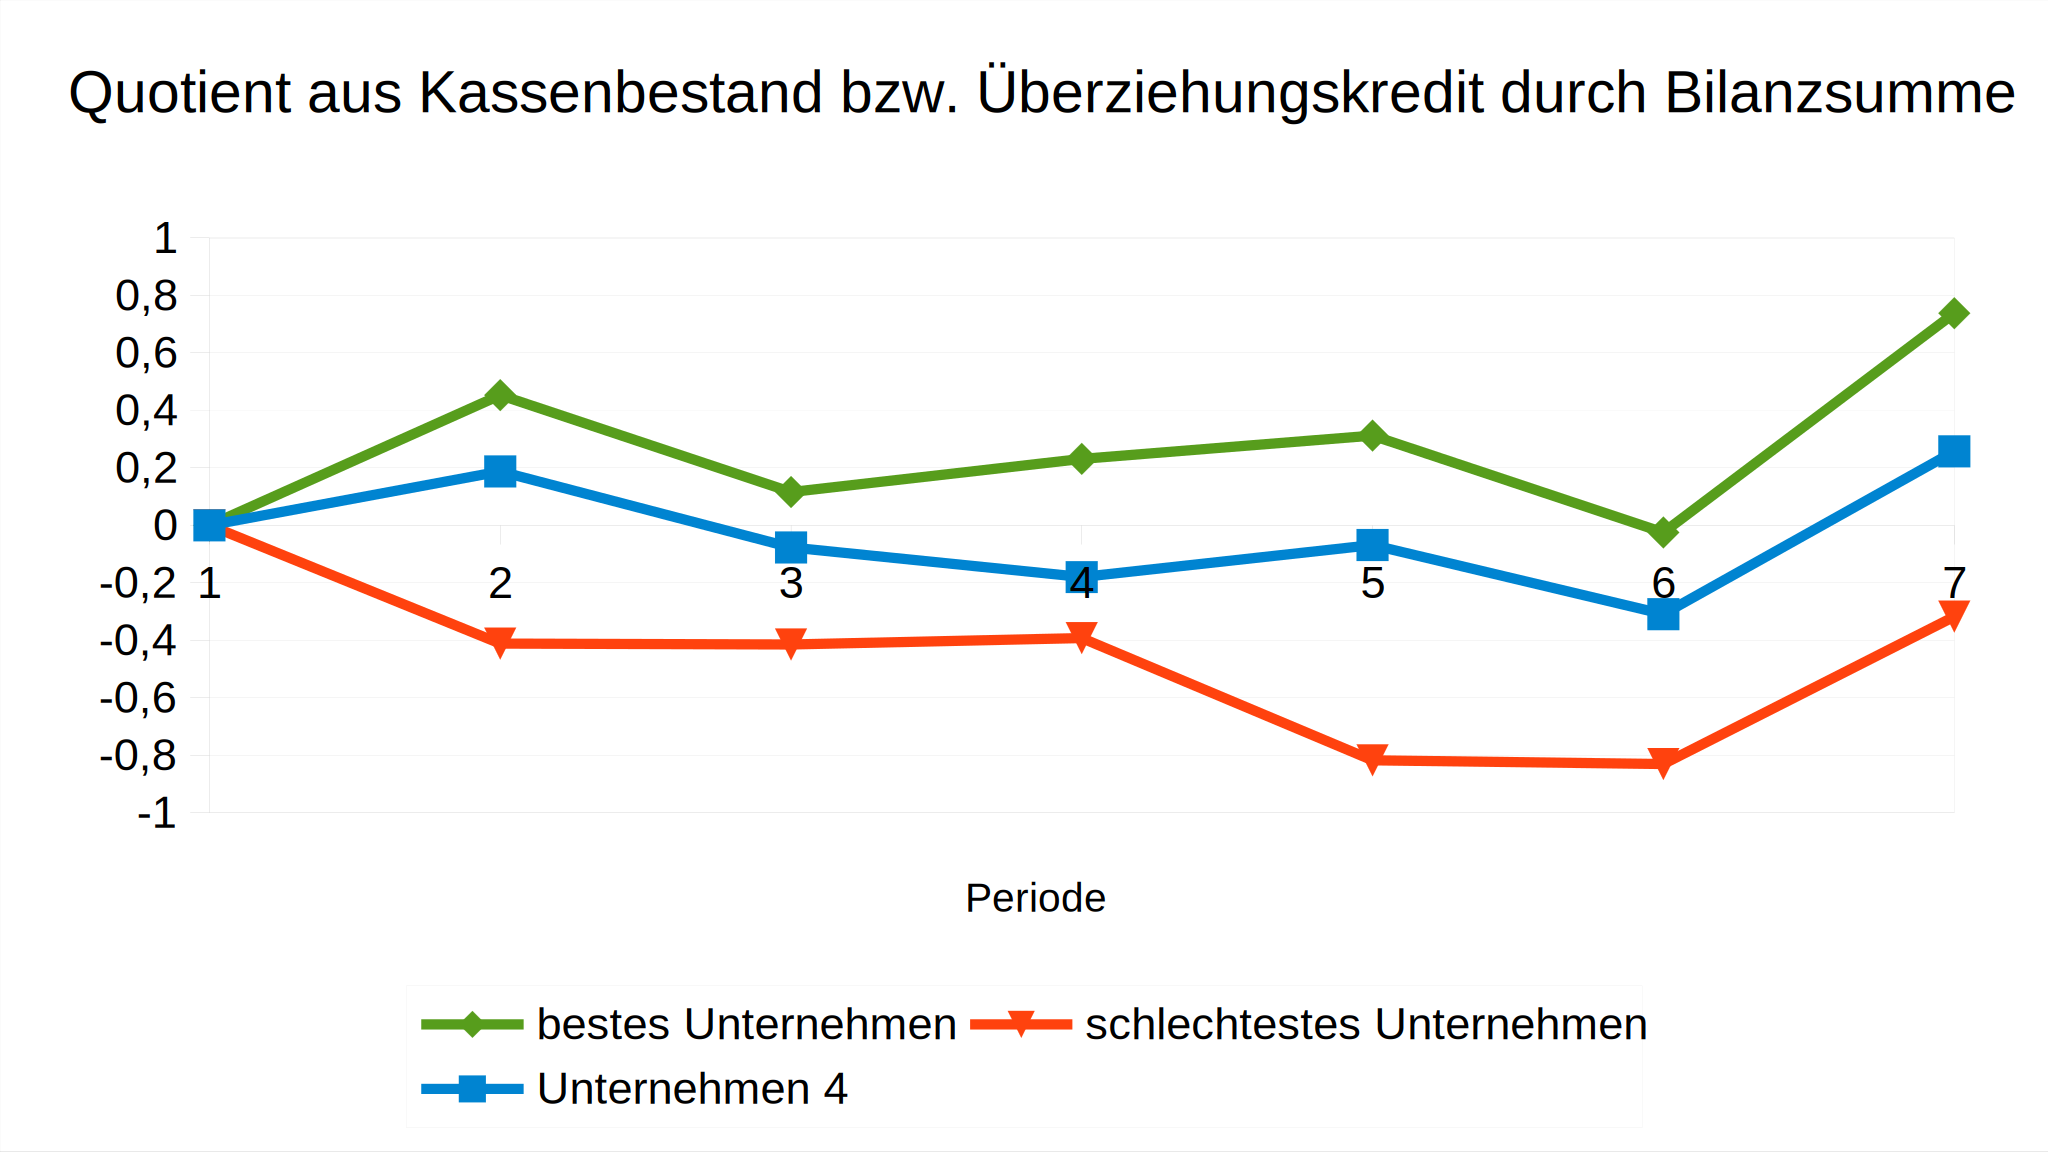
\includepdf[noautoscale]{./img/Quotient.pdf}


\includepdf[noautoscale, pages=-]{./img/Anhang.pdf} 

\includepdf[noautoscale, pages=-]{./img/TopSim_Anhang.pdf}
 
 \listoffigures
 
%
%\begin{figure}[htbp]
%\centering
%\includesvg[width=1\textwidth]{./Herstellkosten}
%	\caption{Herstellkosten}
%%  \caption{svg NewTux}
%\end{figure}
%
%
%\begin{figure}[htbp]
%\centering
%\includesvg[width=1\textwidth]{./kumulierter_Erfolgswert}
%	\caption{kumulierter Erfolgswert}
%%  \caption{svg NewTux}
%\end{figure}
%
%
%\begin{figure}[htbp]
%\centering
%\includesvg[width=1\textwidth]{./kumulierter_Periodenueberschuss}
%	\caption{kumulierter Periodenüberschuss}
%%  \caption{svg NewTux}
%\end{figure}
%
%
%\begin{figure}[htbp]
%\centering
%\includesvg[width=1\textwidth]{./Lagerbestand_an_Fertigprodukten}
%	\caption{Lagerbestand an Fertigprodukten}
%%  \caption{svg NewTux}
%\end{figure}
%
%
%\begin{figure}[htbp]
%\centering
%\includesvg[width=1\textwidth]{./Periodenueberschuss}
%	\caption{Periodenüberschuss}
%%  \caption{svg NewTux}
%\end{figure}
%
%
%\begin{figure}[htbp]
%\centering
%\includesvg[width=1\textwidth]{./Quotient}
%	\caption{Quotient}
%%  \caption{svg NewTux}
%\end{figure}

\chapter{Erklärung}
Hiermit erklären wir, dass der vorliegende Abschlussbericht einschließlich Anlagen von uns in Gemeinschaftsarbeit selbst erstellt wurde und dabei alle Unterzeichner einen annähernd gleichen Anteil erbracht haben.\newline \newline
Aachen, den \today
\newline \newline

Unterschrift 1
\newline \newline
\rule{5cm}{0.4pt}
\\
Sascha Kortemeier
\newline \newline \newline

Unterschrift 2
\newline \newline
\rule{5cm}{0.4pt}
\\
Tobias Weitz
\newline \newline \newline

Unterschrift 3
\newline \newline
\rule{5cm}{0.4pt}
\\
Marcel Hoetz

\end{flushleft}

\end{document}
